\chapter{QUADRO METODOLÓGICO}
\par O quadro metodológico descreve os passos realizados para a 
execução do trabalho. Neste capítulo serão listados, em suas seções, os
itens essenciais no desenvolvimento do trabalho, sendo eles as técnicas, procedimentos, práticas e instrumentos
utilizados, o contexto de aplicação e o tipo de pesquisa.

\section{Tipo de pesquisa}

\par Para \citeonline[p.42]{pesquisa_social_gil}, a pesquisa tem um caráter
pragmático, é um “processo formal e sistemático de desenvolvimento do método científico. 
O objetivo fundamental da pesquisa é descobrir respostas para problemas mediante
o emprego de procedimentos científicos”.

\par Este trabalho terá como base a metodologia de pesquisa aplicada, pois
será desenvolvida uma aplicação inteligente utilizando Algoritmos Genéticos para
o auxílio na tomada de decisão sobre o processo de produção de calças de uma
confecção. Esta pesquisa consiste em procurar respostas para problemas propostos
baseados em padrões e conhecimentos já existentes.

\par \citeonline[p.35]{livro_metodos_de_pesquisa} afirmam que o método de
pesquisa aplicada, "objetiva gerar conhecimentos para aplicação prática, dirigidos a
solução de problemas específicos. Envolve verdades e interesses locais."  

\par Segundo \citeonline{livro_metodologia_de_estudo_de_pesquisa}, a pesquisa
aplicada tem como motivação básica a solução de problemas
concretos, práticos e operacionais e também pode ser chamada de pesquisa
empírica, pois o pesquisador precisa ir a campo, conversar com pessoas e
presenciar relações sociais.

\par Como citam \citeonline{tecnicas_de_pesquisa}, a pesquisa aplicada
caracteriza-se por possuir um interesse prático, quando os resultados serão aplicados ou utilizados na
solução de problemas que ocorrem na realidade, sempre visando gerar conhecimento
para solucionar situações específicas.

\par Como já foi explicado o tipo de pesquisa em que se enquadra este trabalho,
ela deve ser aplicada a um determinado contexto, conforme será explicado na
seção a seguir.

\section{Contexto de pesquisa}

\par Sabe-se que com a alta competitividade no mercado, as empresas, cada vez mais,
buscam diferenciais para seus produtos e, neste cenário, a ideia
de redução de custos se torna essencial, uma vez que tal redução pode ser
refletida no preço dos produtos permitindo que estes se diferenciem dos demais.
Dentre os fatores que viabilizam tais reduções está a otimização de processos que
consiste em organizar os procedimentos relacionados à produção de forma que
estes se tornem mais eficazes.

\par O software desenvolvido neste trabalho visa organizar uma linha de produção
de forma que esta se torne o mais eficiente possível. Será utilizada como
base uma fábrica de confecção de calças situada na cidade de
Cachoeira de Minas - MG, porém a base de conhecimento pode ser aplicada a outros
tipos de negócios que seguem o mesmo padrão de desenvolvimento de produtos.

\par Como cada funcionário trabalha em sua casa, é preciso ter uma boa
forma de distribuir o trabalho, permitindo que a produção possa ser feita em um
tempo menor e com custo reduzido.
Para isso, é necessário que o software faça a distribuição dos lotes a
serem confeccionados entre as costureiras de forma que estas sejam
alocadas de forma a receberem a quantidade de peças de acordo com sua
capacidade de trabalho, considerando também o tempo que cada costureira
irá gastar para pegar as peças e o material necessário para realizar seu
trabalho, além disso o software considera o preço cobrado por cada uma das
delas.

\par A aplicação cruza então todas estas informações de forma a se produzir
soluções para o problema e, no final, a melhor destas soluções será aquela 
que ofereça o menor custo e o menor tempo de produção. Porém, sabe-se que, 
em algoritmos genéticos, não há garantias que a solução encontrada é a melhor
para se resolver o problema mas a tendência é que a solução proposta pelo
algoritmo seja muito boa e seria muito difícil encontrá-la manualmente. 

\section{Instrumentos}

\par Segundo \citeonline{aula_joelma_26_03_15}, instrumentos de pesquisa são a
forma pela qual os dados são coletados para a realização do trabalho, podendo ser,
dentre outras, por meio de reuniões, questionários e entrevistas. Para
este trabalho foi utilizado os instrumentos descritos nas subseções a seguir.

\subsection{Entrevistas}
\par Segundo \citeonline{metodoliga_qualitativas_na_sociologia}, entrevista é
uma interação entre duas pessoas em que uma representa o entrevistador, 
que através de perguntas, obtêm informações por parte de outra pessoa que
representa o entrevistado.


% entrevista é um
% “processo de interação social entre duas pessoas na qual uma delas, o entrevistador,
% tem por objetivo a obtenção de informações por parte do outro, o entrevistado”



\par Foi realizada uma entrevista com o dono da empresa de confecção com o
objetivo de entender seu modelo de negócio para que então fosse possível começar
a fazer o levantamento dos requisitos do sistema. Para
\citeonline[p.128]{pressman2011engenharia}, levantamento de requisitos de
software consiste em

\begin{citacao}
``perguntar ao cliente, aos usuários e aos demais interessados quais são os
objetivos para o sistema ou produto, o que deve ser alcançado, como o sistema ou
produto atenda às necessidades da empresa e, por fim, como o sistema ou produto
deve ser utilizado no dia a dia''.
\end{citacao} 

\par A entrevista ocorreu no dia 09/05/2015 para conhecer mais sobre o processo de 
produção da fábrica. Nesta entrevista, ficou esclarecido todo processo e também
se teve acesso à forma como era controlada a distribuição da produção entre os funcionários. Toda
produção era controlada por meio de planilhas Excel, gerenciadas e alimentadas pelo proprietário. 
Tais planilhas contemplavam as estimativas de produção, as datas de entrega dos
lotes encomendados, levando em consideração a quantidade de peças por lote, o
corte e também o tempo que cada lote levaria para ser entregue.


\subsection{Reuniões}
\par De acordo com \citeonline{ref_reuniao}, reunião é o ajuntamento de
pessoas para se tratar de um determinado assunto em que é necessário que se
tenha conclusões sobre as questões que foram discutidas.

\par Durante o desenvolvimento do trabalho seriam realizadas várias reuniões
com o proprietário da fábrica de calças para sanar as dúvidas, sugestões e
outros assuntos que poderiam surgir. Todavia foi realizada apenas uma reunião com o proprietário
da empresa para poder entender como funciona o processo de produção, pois foi constatado nesta reunião que o
processo de produção havia sido alterado. No processo inicial, o qual foi a base
para este trabalho, cada funcionário trabalhava em sua residência e as peças eram distribuídas entre eles. Atualmente o processo
passou por muitas mudanças, uma delas é que a produção é feita em um lugar
apenas, sem a necessidade de transportar as peças entre as casas dos
funcionários. Segundo o proprietário isso gerou um ganho de tempo bem
expressivo, pois as peças circulavam dentro de um mesmo local e não pela cidade. 

\par Considerando essa mudança, não foram feitas outras reuniões com o
proprietário da fábrica, pois o trabalho não atende mais o processo de produção
atual da fábrica, porém o mesmo pode ser usado em outras empresas que seguem a
forma de produção pesquisada. Assim, foi definido um escopo para o desenvolvimento da aplicação baseando-se no 
processo inicial da fábrica de calças, que se resume em construir uma aplicação levando em consideração que:

\begin{itemize}
	
	\item o processo de desenvolvimento das calças deveria ser dividido em
	atividades com ordem de precedência;
	
	\item cada atividade poderia ser feita por uma ou mais costureiras, de acordo
	com a habilidade de cada uma;
	
	\item cada costureira gasta um tempo, medido em segundos, para fabricar uma
	peça;
	
	\item cada costureira cobra um preço por peça produzida;
	
	\item o usuário deveria ser capaz de cadastrar um novo processo, costureiras e
	habilidades;
	
	\item o usuário deveria cadastrar o tempo e o preço de produção, por peça, para
	cada costureira além de sua posição geográfica; 
	
	\item o total de peças deveria ser dividido em lotes e cada costureira deveria
	receber uma quantidade de lotes distribuída aleatoriamente;
	
	\item o usuário deveria informar uma data de entrega das peças de um processo e
	uma data de início de execução do mesmo para que se pudesse calcular o prazo;
	
	\item o software deveria então oferecer como saída a melhor distribuição de
	forma a se produzir no menor tempo dentro do prazo, com o menor custo, considerando 
	o tempo e o preço de produção de cada costureira e o tempo de transporte das peças 
	entre elas.
	
	\item se o software não conseguisse encontrar nenhuma solução abaixo do prazo, a
	busca pelo menor custo seria ignorada e o menor tempo encontrado seria retornado.
	
\end{itemize}

\par A seção a seguir descreve como foi definido o escopo demonstrado acima.

\section{Procedimentos}

\par Esta seção descreve os procedimentos realizados na execução do trabalho,
definindo primeiramente o \textit{framework} de desenvolvimento e explicando
como o algoritmo genético foi desenvolvido para os requisitos definidos no escopo.

\subsection{Framework de desenvolvimento}
\par Primeiramente é necessário ressaltar que, para o desenvolvimento da aplicação, foi utilizada uma base desenvolvida pelo professor Artur Barbosa durante as aulas de sistemas especialistas, do VII período do curso de sistemas de informação nesta universidade.
Esta base também denominada \textit{framework}, define regras a serem seguidas no desenvolvimento de cada elemento
de um algoritmo genético. Tal \textit{framework} é definido dentro da seguinte estrutura:

\begin{itemize}
	
	\item Classe \texttt{GAModel}:
	\par A classe \texttt{GAModel} é basicamente a classe mãe de todos os elementos de um algoritmo genético, 
	que representa o modelo que irá armazenar a população de indivíduos além de ser
	a classe que armazena os parâmetros que definem as configurações do algoritmo, tais como, tipo de cruzamento, tipo de mutação, 
	tamanho da população etc.
	
	\par A classe contém os seguintes atributos:
	
	\begin{itemize} 
		\item \textit{populationSize}:
		este atributo define qual será o tamanho da população, ou seja, quantos
		indivíduos irão formar cada população;
		
		\item \textit{generationQuantity}:
		como já explicado no quadro teórico, o processo de cruzamento e mutação se
		repete até que o número de indivíduos, definido no atributo anterior, seja atingido formando assim uma nova população e então, por sua vez, 
		este processo de geração de novas populações se repete até que seja atingido um número de gerações definido 
		pelo programador. Este atributo representa esta quantidade;
		
		\item \textit{elitism}:
		atributo do tipo \textit{boolean} que representa se o algoritmo vai ter a
		função de elitismo.
		Esta função, como já foi explicada no quadro teórico, quando está ativada (com
		valor \textit{true}), no momento de começar a se criar uma nova população os dois melhores indivíduos da população que será 
		substituída já começam a fazer parte da nova população, antes de começar o processo de cruzamento e mutação. 
		Este mecanismo garante que a nova população terá pelo menos dois indivíduos iguais ao da antiga população, o que irá 
		impedir que a nova população não seja pior que a anterior;
		
		\item \textit{foreignIndividualRate}:
		este atributo define a taxa de novos indivíduos que devem entrar em novas
		populações e será visto com mais detalhes na seção Indivíduos Estrangeiros.
		
		\item \textit{mutationRate}:
		como descrito no quadro teórico, a mutação é o fato de realizar pequenas
		alterações no indivíduo a fim de que este possa se tornar ainda melhor. Este parâmetro define uma porcentagem, geralmente baixa, que define quando 
		o indivíduo sofrerá mutação ou não. Esta questão ficará mais clara logo
		abaixo, quando será explicado o passo-a-passo da execução do algoritmo.
		
		\item \textit{mutationQuantity}:
		caso a mutação for ocorrer para o indivíduo, a alteração aleatória será feita
		nos cromossomos.
		Este parâmetro define quantos cromossomos do indivíduo deve ser alterado pela mutação;
		
		\item \textit{selectionType}:
		conforme descrito no quadro teórico, existem várias formas de seleção dos
		indivíduos para realizarem o cruzamento. Este parâmetro define qual será a forma escolhida pelo programador ao
		implementar o seu problema.No \textit{framework} este parâmetro é do tipo \texttt{enum} e pode assumir 2 valores o
		\textit{ROULETTE}, que define que o método de seleção utilizado será o de roleta e o \textit{CLASSIFICATION}, que 
		define que o método a ser utilizado é o de classificação. Neste projeto o
		método padrão que já foi pré-definido no código foi o método de roleta;
		
		\item \textit{crossType}:
		Assim como a seleção, existe diversas formas de fazer o cruzamento dos indivíduos. Este atributo, 
		também do tipo \texttt{enum} representa a forma de cruzamento e pode receber os valores \textit{Binary}, 
		\textit{Permutation}, \textit{Uniform} e \textit{Aritmetic}, esses valores
		definem qual implementação de cruzamento o algoritmo deve utilizar, esta aplicação
		utilizará o método \textit{Permutation}, desta forma somente um
		método de cruzamento foi implementado conforme mostra a seção Seleção,
		cruzamento e mutação;
		
		\item \textit{mutationType}:
		Segue a mesma forma que o selectionType e o crossType e pode assumir os valores \textit{Permutation}, 
		\textit{Binary} e \textit{Numerical}, e neste projeto foi o escolhido o
		método \textit{Permutation}.
		
	\end{itemize}
	
	\item Classe \texttt{Individual}:
	\par A classe abstrata \texttt{Individual} representa a estrutura básica de um indivíduo. 
	A classe contém uma \texttt{lista} do tipo 
	\texttt{Cromossomo}, que será descrita posteriormente, que contém uma coleção
	de objetos que representam as características da solução.
	
	\par A Classe contém ainda um atributo chamado \texttt{valor} que irá armazenar a qualidade, ou seja, qual é o custo
	da solução representada pelo indivíduo, tal valor é recebido no retorno da
	operação \texttt{calculateValue()} descrita abaixo.
	
	\par Com relação as operações, além dos \textit{getters and setters}, a classe contém a operação abstrata 
	\texttt{calculateValue()}, que realiza a função de avaliação, que mede a qualidade do indivíduo. Desta forma, ao utilizar este \textit{framework}, a classe que representa o indivíduo do 
	problema deve herdar desta classe  \texttt{Individual}. Fazendo isso, tal classe passará a ter uma lista de cromossomos 
	e o atributo que representa o seu valor e a classe obrigatoriamente terá que implementar a operação 
	\texttt{calculateValue()}, permitindo assim que o programador 
	desenvolva a função de avaliação específica para o seu problema.
	
	
	\item Classe \texttt{Chromosome}:
	\par É uma classe abstrata, que possui todos os métodos abstratos, desta forma
	ela só existe para garantir que os cromossomos do problema irão implementar os
	métodos necessários para o funcionamento do algoritmo. Estes métodos são:
	
	\begin{itemize}
		
		\item \texttt{equals}: necessário para efeito de comparação dos cromossomos;
		
		\item \texttt{doMutation}: realiza a mutação. Este deve
		ser implementado pela classe que representa o cromossomo, pois a
		mutação é feita nos cromossomos.
		
		\item \texttt{clone}: devolve um objeto exatamente com os mesmos
		atributos do objeto, porém em uma instância diferente.
		
	\end{itemize}
	
	
	\item Classe \texttt{IndividualPair}:
	\par A classe \texttt{IndvidualPair} possui uma estrutura simples. Apenas
	representa dois indivíduos. Ela se torna necessária, pois o processo de
	cruzamento dos indivíduos retornam dois novos indivíduos, desta forma, como 
	no Java não é possível retornar dois valores, é retornado então um objeto desta
	classe contendo os dois novos indivíduos criados. 
	
	
	\item Classe \texttt{GAController}:
	\par A classe \texttt{GAController}, como o próprio nome já diz, é o
	controlador de todo processo de execução do algoritmo genético.
	Ela recebe no seu construtor o modelo que é do tipo \texttt{GAModel}, que como
	já explicado anteriormente, armazena os parâmetros a serem seguidos na
	execução do algoritmo. Além disso, através do seu método principal
	denominado \texttt{execute()}, ela é responsável por criar novas populações, a
	partir de cruzamentos, mutações, elitismo, etc, tendo também a
	responsabilidade de chamar a função de classificação e avaliação de cada indivíduo.
	
	\par Os pontos a seguir descrevem basicamente os passos executados dentro do
	método execute(). Outros detalhes serão vistos mais adiante quando será
	descrita a implementação do algoritmo da fábrica de calças, pois será
	necessário realizar algumas adaptações neste \textit{framework}.
	
	\begin{itemize}
		\item	Criação da população inicial, através do método createInitialPopulation()
		do objeto que será extendido da classe GAModel;
		
		\item Classificação e avaliação da população inicial através do método
		\texttt{classify()};
		
		\item Realização do processo de elitismo, através do método
		\texttt{doElitism()};
		
		\item Inserção de indivíduos estrangeiros na população;
		
		\item Realização do processo de seleção de indivíduos, através do método
		\texttt{doSelection()};
		
		\item Execução do processo de cruzamento e mutação, através do método
		\texttt{doCrossing()} e \texttt{doMutaion()} respectivamente.
		
		
	\end{itemize}
	
	\par Após estes passos, uma nova população foi criada e está
	armazenada na variável newGeneration, assim o método
	\texttt{setPopulation()} do objeto \texttt{model} é chamado para então substituir
	a antiga população pela nova. Como a execução está dentro de uma estrutura de repetição
	\texttt{for}, ocorre um \texttt{loop} e então é recomeçado o processo de
	criação de uma outra população. Este processo para quando o número de gerações, 
	definido no parâmetro \texttt{generationQuantity} do objeto \texttt{model}
	for atingido, neste caso é dado o comando \texttt{break} e o \texttt{loop} é encerrado.
	% 	Para começar é chamado o método  \texttt{createInitialPopulation} da classe
	% 	\texttt{GAModel} para criar a população de indivíduos, este método será
	% 	implementado pela classe que irá herdar da classe \texttt{GAModel}.
	
	% 	\par Cada indivíduo representa uma solução para o problema, sua estrutura é
	% 	composta pela parte da calça a ser produzida, a costureira com
	% 	habilidade para produzir essa peça e o numero de lotes sorteados a ela.
	% 	Para explicar melhor precisa-se produzir um lote de 500 peças, será preciso
	% 	produzir 500 partes da frente, 500 partes de traz, etc., e assim
	% 	sucessivamente.
	% 	Esse lote de 500 peças é divdido entre os indivíduos da população. Para um
	% 	melhor entender a estrutura de um indivíduo veja a figura 5 a seguir:
	% 	
	% 	\begin{figure}[h!]
	% 	\centerline{\includegraphics[scale=0.5]{./imagens/individuos.png}}
	% 	\caption[Representação da estrura de um indivíduo]
	% 	{Representação da estrura de um indivíduo \textbf{Fonte:} Desenvolvido pelos autores}
	% 	\label{fig:exemplo1}
	% 	\end{figure} 
	
	
	
\end{itemize}

\par As próximas seções apresentam a implementação dos requisitos da aplicação
e dos elementos do algoritmo genético, seguindo as definições do \textit{framework}.

\subsection{Representação do processo de produção}

\par Primeiramente foi definido como seria o processo de fabricação. Este foi pensado com base no 
processo da fábrica, em que a confecção das peças deveria ser dividida em atividades que representam
cada parte da calça. Neste contexto, surgiu a necessidade de determinar uma ordem para a execução do processo, 
devido ao fato de que algumas atividades dependem da finalização de outras para poderem ser
realizadas. A Figura ~\ref{fig:processo_fabricacao} demonstra basicamente um
exemplo de ordem de execução do processo de confecção.


\begin{figure}[h!]
	\centerline{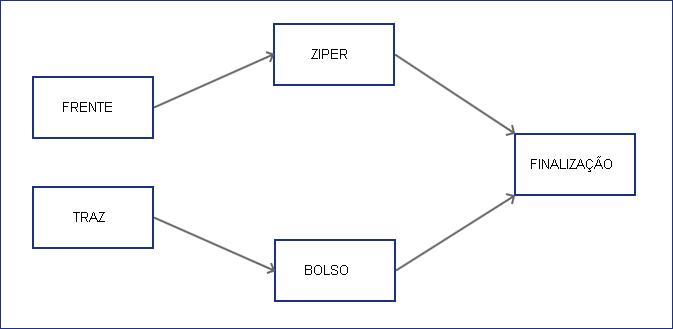
\includegraphics[scale=0.5]{./imagens/processo1.png}}
	\caption[Demonstração de um processo de fabricação]
	{Demonstração de um processo de fabricação \textbf{Fonte:} Desenvolvido pelos
	autores.}
	\label{fig:processo_fabricacao}
\end{figure}

\par  Uma questão importante que foi definida é que, independente da complexidade e tamanho do processo, este deve sempre começar 
com a atividade Carimbo e finalizar com a atividade Finalização. Isso ocorre pois a Finalização é sempre a última atividade 
de qualquer processo da fábrica e o Carimbo é uma atividade simbólica que representa o fato de o dono da fábrica separar o 
material de costura. O tempo e o custo gastos nesta separação não são contabilizados no algoritmo genético, somente o tempo de 
transporte dos materiais até as costureiras são considerados na distribuição, além disto esta atividade terá somente uma pessoa
trabalhando que, neste caso será o Marcelo, dono da fábrica, que é o responsável por este trabalho.

\par Para armazenar este processo e suas atividades no software, foram utilizadas tabelas do banco de dados, conforme mostra 
a Figura ~\ref{fig:proc_fabri_db}.

\newpage

\begin{figure}[h!]
	\centerline{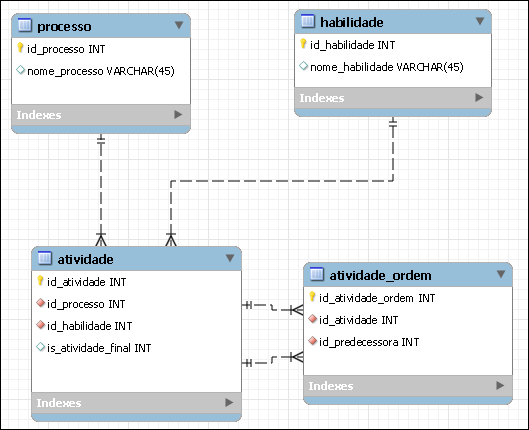
\includegraphics[scale=0.7]{./imagens/representacao_processo.png}}
	\caption[Representação do processo de fabricação no banco de dados]
	{Representação do processo de fabricação no banco de dados \textbf{Fonte:}
	Desenvolvido pelos autores.}
	\label{fig:proc_fabri_db}
\end{figure}

\par A tabela \texttt{processo} tem como finalidade gerar um código único para representar 
cada processo de produção, cada processo representa um modelo, cada modelo
de calça possui um processo diferente que pode possuir diferentes atividades que
são representadas na tabela \texttt{atividade}, onde é feita a relação que define quais são as atividades de 
um processo,  além de conter quais são as habilidades necessárias para cada atividade, ou seja, cada registro desta 
tabela representa uma atividade do processo e qual habilidade é necessária para sua execução. O campo 
\texttt{is\_atividade\_inicial}, quando tem o valor 1, define que tal atividade
é a atividade Finalização. Esta \textit{flag} é importante no momento de calcular o tempo total de execução do
processo e será visto com mais detalhes posteriormente e, por fim, a tabela
\texttt{atividade\_ordem} é onde é feita a definição de ordem de execução das
atividades.

\par A Figura ~\ref{fig:class_atividadeOrdem} demonstra o mapeamento da relação
entre a tabela \texttt{atividade} e atividade\_ordem para o Java.

\newpage

\begin{figure}[h!]
	\centerline{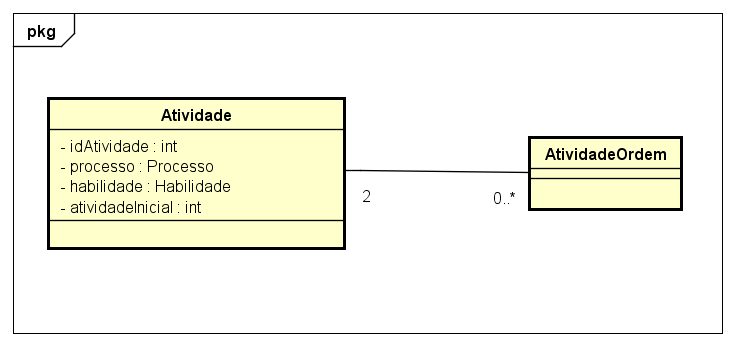
\includegraphics[scale=0.7]{./imagens/atividade_diagram.png}}
	\caption[Classes Atividade e AtividadeOrdem]
	{Classes Atividade e AtividadeOrdem \textbf{Fonte:} Desenvolvido pelos
	autores.}
	\label{fig:class_atividadeOrdem}
\end{figure} 

\par A classe Atividade pode ter zero ou vários objetos da classe
AtividadeOrdem.
Esta possui dois objetos da própria classe Atividade, um representando uma
atividade e outro representando a sua predecessora.

\par Considerando o processo de produção e o modelo de dados apresentados acima, foi
desenvolvido um algoritmo genético para a solução do problema de otimização. Conforme já demonstrado 
no Quadro Teórico, um algoritmo genético deve seguir uma ordem de execução conforme mostra
a Figura ~\ref{fig:exec_ag}.


\begin{figure}[h!]
	\centerline{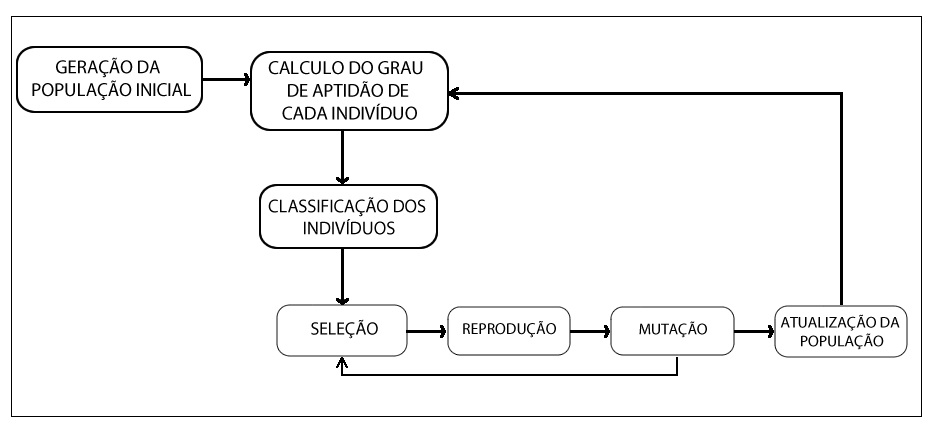
\includegraphics[scale=0.6]{./imagens/algoritimos_geneticos.jpg}}
	\caption[Demonstração da execução de um AG]
	{Demonstração da execução de um AG \textbf{Fonte:} Desenvolvido pelos autores.}
	\label{fig:exec_ag}
\end{figure}

\newpage


\par O primeiro passo para a execução do algoritmo então foi o desenvolvimento de uma lógica para a criação
da população inicial de indivíduos, conforme explicado na próxima seção.

\subsection {População inicial: Distribuição das atividades, Indivíduos e Cromossomos}

\par Para um melhor entendimento dos conceitos a serem explanados, é necessário
conhecer, de forma básica, o fluxo de execução da aplicação. Como será visto na seção que descreve a construção
da interface gráfica, o usuário irá iniciar a execução do algoritmo genético através de uma tela de distribuição de atividades, nesta tela ele deve informar o número de peças que deseja produzir, a quantidade de peças que cada lote deve possuir e uma data de início das atividades. Através da data de início e a data de entrega, informada no cadastro do processo, o controlador da tela calcula o prazo de entrega e o número total de lotes e chama o serviço de gerenciamento da execução do AG, passando o número de lote, o número de peças por lote e o prazo de entrega a ser considerado durante a distribuição. Tal serviço, por sua vez, configura os parâmetros do algoritmo genético e da início a execução deste. A Figura ~\ref{fig:fluxo_basico} ilustra o fluxo básico de execução da aplicação.

\begin{figure}[h!]
	\centerline{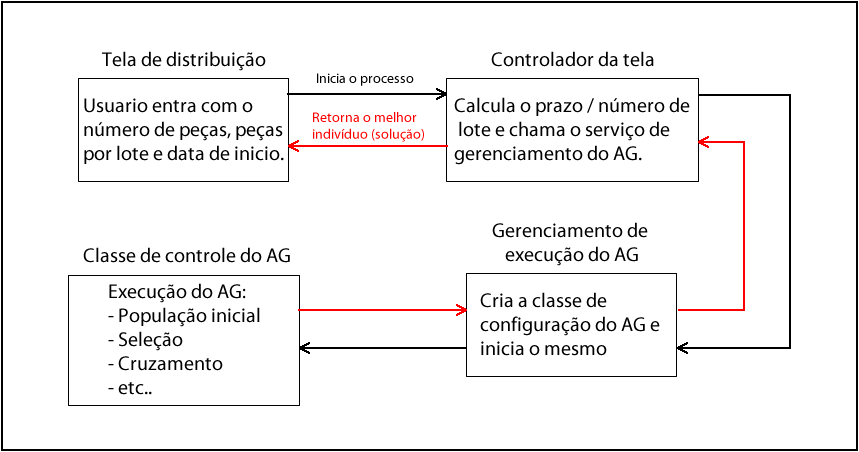
\includegraphics[scale=0.5]{./imagens/fluxo_basico.png}}
	\caption[Demonstração da execução de um AG]
	{Fluxo básico de execução \textbf{Fonte:} Desenvolvido pelos autores.}
	\label{fig:fluxo_basico}
\end{figure}

\par Conforme ilustrado na Figura ~\ref{fig:fluxo_basico}, o processo de criação da população inicial assim como o processo de seleção, 
cruzamento e mutação e a chamada da função de avaliação de cada indivíduo, ocorre dentro dentro de uma classe de controle,
ou seja, esta classe faz a orquestração de toda a execução do AG. Tal classe é denominada \texttt{GAController} e
pertence ao \textit{Framework} explanado anteriormente.

\par A classe criada para o gerenciamento da execução do algoritmo genético é denominada \texttt{GeneticAlgorithmManagement} e, conforme demonstrado na Figura ~\ref{fig:fluxo_basico}, esta é instanciada pelo controlador da tela de distribuição de atividades. Tal classe possui 
um único método denominado \texttt{iniciarDistribuicao()} e recebe neste os dados informados pelo usuário, além disto, neste
método, é criado um objeto de \texttt{ProcessoModel}, que herda da classe \texttt{GAModel} do \textit{framework}, e, neste, são 
definidos os parâmetros a serem usados pelo algoritmo genético, além disso, os dados informados pelo usuário também são definidos 
neste objeto pois são utilizados pela regra de negócio seguida na execução do AG. O Código \ref{list:iniciarDistribuicao} 
demonstra o método \texttt{iniciarDistribuicao()}.


\begin{lstlisting} [style=custom_Java,caption={[Métodos da classe
\texttt{FilmeBean}]{Método \texttt{iniciarDistribuicao()} da classe \texttt{GeneticAlgorithmManagement}. \textbf{Fonte:}
Elaborado pelos autores.}}, label=list:iniciarDistribuicao]

public ProcessoIndividual iniciarDistribuicao(
			int numeroLote,BigDecimal prazEmSegundos,  
			int pecasPorLote,int idProcesso){

		EntityManager manager = ConFactory.getConn(); 
		
		ProcessoModel model = new ProcessoModel(manager,idProcesso);
		model.setNumeroLote(numeroLote);
		model.setPecasPorLote(pecasPorLote);
		model.setPrazoEmSegundos(prazEmSegundos);
		model.setGenerationQuantity(10000);
		model.setPopulationSize(80);
		model.setElitism(true);
		model.setSelectionType(GAModel.SelectionType.CLASSIFICATION);
		model.setCrossType(CrossType.PERMUTATION);
		model.setForeignIndividualRate(0.3f);
		model.setMutation(GAModel.MutationType.PERMUTATION);
		model.setMutationRate(0.05f);
		model.setMutationQuantity(1);

		GAController controller = new GAController(model);
		return (ProcessoIndividual) controller.execute();
}


\end{lstlisting}

\par Tal método retorna um objeto do tipo \texttt{ProcessoIndividual} para o controlador da tela de distribuição, este é o melhor indivíduo encontrado, ou seja, a melhor solução encontrada. Tal solução será então apresentada ao usuário conforme mostra a Figura ~\ref{fig:fluxo_basico}.

\par A classe \texttt{ProcessoModel}, ao ser instanciada, recebe em seu construtor uma conexão para o 
banco de dados e o \texttt{ID} do processo a qual será executado o algoritmo. O construtor desta então chama o método
\texttt{getInformacoesCostureiras()} que tem por finalidade buscar no banco de dados todas as atividades do processo em questão, 
buscar todas as costureiras que tem a habilidade de fazer cada uma destas e criar um \texttt{HashMap} que possui como chave o 
\texttt{ID} da atividade e como valor uma lista de \texttt{CostureiraHabilidade}, feito isto o método também recupera  a 
atividade final (Finalização), conforme demonstra o Código ~\ref{list:getInformacoesCostureiras}.


\begin{lstlisting} [style=custom_Java,caption={[Métodos da classe
\texttt{FilmeBean}]{Método \texttt{getInformacoesCostureiras}. \textbf{Fonte:}
Elaborado pelos autores.}}, label=list:getInformacoesCostureiras]

public void getInformacoesCostureiras() {
	List<CostureiraHabilidade> costureirasHabilidades = null;
	
	if (atividadesCostureiras != null && atividadesProcesso != null){
	   atividadesCostureiras.clear();
	   atividadesProcesso.clear();
	}
	
	atividadesCostureiras = 
	   new HashMap<Integer, List<CostureiraHabilidade>>();
	
	atividadesProcesso = 
	   atividadeDao.listAtividadesByProcesso(processo);
	
	/* Montar um MAP tendo como chave cada atividade do processo 
	   e a lista de costureiras que tenham a habilidade relacionada.*/
	for (Atividade atividade : atividadesProcesso) {
		
		costureirasHabilidades = 
		   cdao.getCostureirasByHabilidade
		      (atividade.getHabilidade().getIdHabilidade());
		
		atividadesCostureiras.put
		   (atividade.getIdAtividade(),costureirasHabilidades);
		
		if (atividade.isAtividadeFinal()) atividadeFinal = atividade;
	}
}

\end{lstlisting}

\par Então, após a definição dos parâmetros, é criado um novo objeto de \texttt{GAController} passando-se o 
objeto da classe \texttt{ProcessoModel} com todos os parâmetros do algoritmo genético, os dados do usuário e 
informações de atividades e costureiras do processo em questão e então  o método \texttt{execute()} é chamado, dando-se início  
a execução do algoritmo genético. A primeira coisa a ser feita então é criar a população inicial de indivíduos que é criada a  partir do método \texttt{createInitialPopulation()} declarado de forma abstrata na classe \texttt{GAModel} e implementado pela classe 
\texttt{ProcessoModel}. Tal método basicamente executa um \texttt{for} de 0 até o tamanho da população (atributo 
\texttt{populationSize}) e assim para cada iteração é criado um objeto de \texttt{ProcessoIndividual} passando a 
\texttt{atividadeFinal}, o \texttt{map} que contém as atividades e suas costureiras (\texttt{atividadesCostureiras}) criados 
pelo método \texttt{getInformacoesCostureiras()}, além dos atributos \texttt{numeroLote}, \texttt{pecasPorLote} e
\texttt{prazoEmSegundos}, conforme mostra o código ~\ref{list:createInitialPopulation}.


\begin{lstlisting} [style=custom_Java,caption={[Métodos da classe
\texttt{FilmeBean}]{Método \texttt{createInitialPopulation}. \textbf{Fonte:}
Elaborado pelos autores.}}, label=list:createInitialPopulation]

@Override
	public void createInitialPopulation() {
		for (int i = 0; i < getPopulationSize(); i++) {
			population.add
			   (new ProcessoIndividual
			       (atividadeFinal, prazoEmSegundos, atividadesCostureiras,
			        this.numeroLote, this.pecasPorLote));
	}
}

\end{lstlisting}

\par Quando se cria um novo indivíduo, a partir da instanciação de um novo objeto de \texttt{ProcessoIndividual},
acontece então, no construtor da classe, a distribuição das atividades de forma a representar uma solução para o problema.
A realização desta distribuição foi realizada considerando que o total de
peças a ser produzido deveria ser dividido em lotes e então, em cada atividade,
este número de lote deveria ser distribuído entre as costureiras que possuíssem a habilidade em questão. Por exemplo: se a quantidade total de peças de uma ordem de produção for 500,
primeiramente deve-se definir qual será o número de peças por lote, neste caso, se for definido que cada lote  
deverá ter 50 peças, então o resultado final será 500/50 ou seja 10 lotes contendo 50 calças cada um. 

\par Neste sentido, seguindo o exemplo apresentado  na Figura
~\ref{fig:processo_fabricacao}, a distribuição deverá ser feita de forma que para cada atividade do processo seja 
distribuído o trabalho de 10 lotes, ou seja, o material para a confecção de 10 lotes deve ser enviado para as costureiras
que irão fazer a parte da frente e posteriormente estas enviam os 10 lotes para as costureiras que fazem a finalização.

\par Com base nesses requisitos, para a realização de tal distribuição, inicialmente, o algoritmo irá distribuir, 
de forma aleatória, o número de lotes definido entre as costureiras de cada atividade,
conforme mostra a Figura ~\ref{fig:distribuicao_lotes_costureiras}.

\newpage

\begin{figure}[h!]
	\centerline{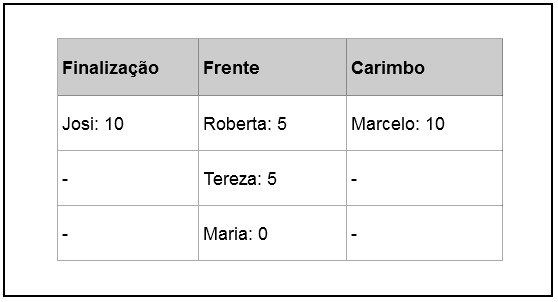
\includegraphics[scale=0.6]{./imagens/distribuicao_exemplo.png}}
	\caption[Exemplo de distribuição aleatória de lotes para as costureiras]
	{Exemplo de distribuição aleatória de lotes para as costureiras \textbf{Fonte:}
	Desenvolvido pelos autores.}
	\label{fig:distribuicao_lotes_costureiras}
\end{figure}

\par Uma costureira pode não receber lote (:0), isso permite que a decisão de
quem vai participar ou não também fique por conta do algoritmo. O exemplo demonstrado está considerando que se irá produzir 500 peças em lotes de 50, 
resultando assim em um total de 10 lotes.

\par Como já explanado no quadro teórico, a estrutura do algoritmo genético é composta
por populações que são formadas por indivíduos que por sua vez são formados por cromossomos.
Cada indivíduo representa uma solução e cada cromossomo do indivíduo representa uma de suas características. 
Assim, então, é gerada uma população inicial de indivíduos e, a partir desta, um
processo de cruzamento e mutação é iniciado a fim de que possam ser gerados
novos indivíduos que representem soluções ainda melhores que seus antecessores.

\par Neste sentido, para o desenvolvimento do algoritmo de distribuição de
lotes, o processo de definição de indivíduo e cromossomo foi o primeiro passo do desenvolvimento da aplicação. Isso se
deve ao fato de que estes elementos compõe a parte crucial para que se
possa definir a lógica a ser seguida para a definição da população inicial, o
tipo de cruzamento, a função de avaliação, etc.

\par Neste caso, cada indivíduo da população irá representar uma forma de
distribuir as atividades e cada número de lotes distribuídos a determinada
costureira em uma determinada atividade irá representar um cromossomo. 
Tomando como base o exemplo da Figura ~\ref{fig:distribuicao_lotes_costureiras},
o quadro, como um todo, representa o indivíduo e cada distribuição, como por exemplo a Roberta, que recebeu 5 
lotes para confeccionar, representa um cromossomo.

\par Para fazer esta representação em Java, primeiramente foi criado uma classe denominada \texttt{ProcessoChromosome} que é
representada na Figura ~\ref{fig:class_processoChromosome}:

\newpage

\begin{figure}[h!]
	\centerline{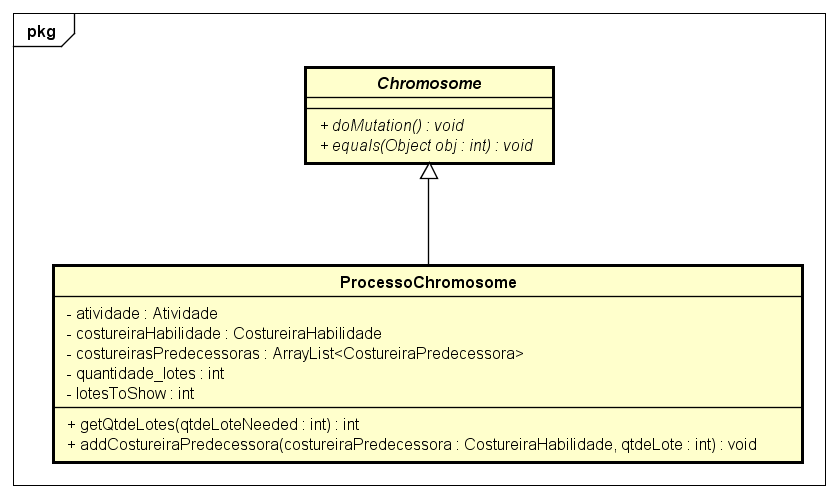
\includegraphics[scale=0.5]{./imagens/processo_chromosome_diagram.png}}
	\caption[Classe ProcessoChromosome]
	{Classe ProcessoChromosome \textbf{Fonte:} Desenvolvido pelos autores.}
	\label{fig:class_processoChromosome}
\end{figure}


\par A classe \texttt{ProcessoChromosome} herda de \texttt{Chromosome} do
\textit{framework} descrito na Figura ~\ref{fig:class_processoChromosome}. Por
enquanto, é necessário compreender apenas os atributos \texttt{atividade}, costureiraHabilidade e
\texttt{quantidade\_lotes}, que recebem seus valores pelo construtor, os
demais atributos e métodos são utilizados pela função de avaliação e serão explicados mais adiante. 
O atributo atividade é do tipo \texttt{int} e representa o \texttt{ID} da
atividade, no banco de dados, a qual se está atribuindo a costureira e a
quantidade de lotes, este atributo será passado na criação de cada cromossomo
sempre que for necessário se criar um novo indivíduo. O atributo \texttt{costureiraHabilidade} 
é do tipo CostureiraHabilidade, que representa o mapeamento da tabela costureira\_habilidade do banco de dados, 
e faz a relação entre quais habilidades cada costureira possui além do tempo e o preço de cada uma para 
fazer uma peça de uma determinada parte da calça, conforme demonstra a Figura ~\ref{fig:dados_costureiras}.


\begin{figure}[h!]
	\centerline{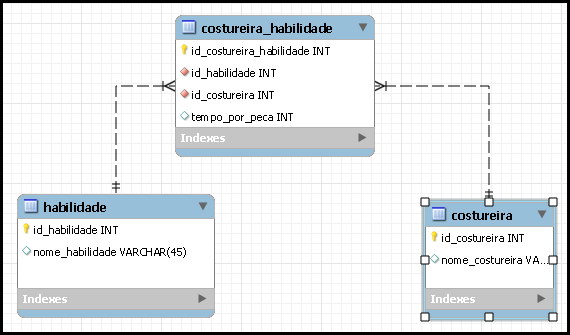
\includegraphics[scale=0.6]{./imagens/costureira_habilidade_tabela.png}}
	\caption[Armazenamento de dados das costureiras]
	{Armazenamento de dados das costureiras \textbf{Fonte:} Desenvolvido pelos
	autores.}
	\label{fig:dados_costureiras}
\end{figure}


\par A classe \texttt{CostureiraHabilidade}, conforme ilustra a Figura
~\ref{fig:class_costureiraHabilidade}, por sua vez, possui o atributo habilidade, outro que
representa a costureira e um terceiro para representar o tempo que tal
costureira gasta para confeccionar uma peça com certa habilidade. Fez-se
necessário ter um atributo da classe CostureiraHabilidade ao invés de simplesmente ter um objeto do tipo Costureira, pois, 
na função de avaliação, como será visto mais adiante, necessita ter o tempo
que a costureira gasta para fazer a peça e este tempo pode variar para uma mesma costureira dependendo de suas habilidades.

\begin{figure}[h!]
	\centerline{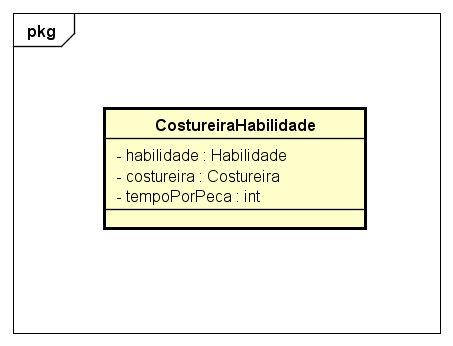
\includegraphics[scale=0.9]{./imagens/costureiraHabilidade_class.png}}
	\caption[Classe CostureiraHabilidade]
	{Classe CostureiraHabilidade \textbf{Fonte:} Desenvolvido pelos autores.}
	\label{fig:class_costureiraHabilidade}
\end{figure}

\par Assim, para representar cada característica da solução, tomando como
exemplo a Figura ~\ref{fig:distribuicao_lotes_costureiras}, o fato de Roberta
fazer 5 lotes da parte da frente é representado na implementação do código criando se um objeto da classe \texttt{ProcessoChromosome} passando no
construtor o \texttt{id} da atividade ``Frente'', um objeto de
\texttt{costureiraHabilidade}, cujo atributo \texttt{costureira} represente a
Marta, o atributo \texttt{habilidade} que representa a habilidade em questão e a
quantidade de lotes que Marta deverá confeccionar, que seria, neste caso, cinco.

\par A representação do indivíduo foi feita criando-se a classe \texttt{ProcessoIndividual} 
como demonstra a Figura ~\ref{fig:class_processoIndividual}:


\begin{figure}[h!]
	\centerline{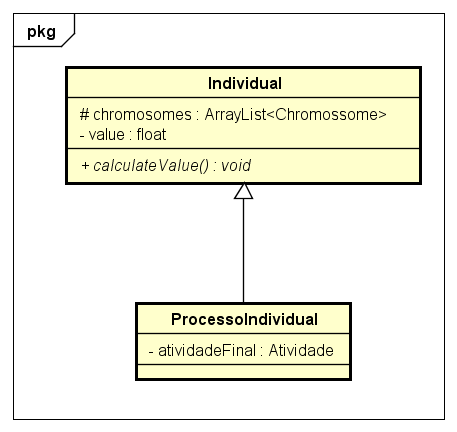
\includegraphics[scale=0.9]{./imagens/class_individual.png}}
	\caption[Classe ProcessoIndividual]
	{Classe ProcessoIndividual \textbf{Fonte:} Desenvolvido pelos autores.}
	\label{fig:class_processoIndividual}
\end{figure}

\par A classe \texttt{ProcessoIndividual} herda da classe \texttt{Individual} do
\textit{framework}, e por isso, esta passa a ter um \texttt{ArrayList} com
objetos do tipo \texttt{Chromosome}. Neste caso, como a classe \texttt{ProcessoChromosome} herda de \texttt{Chromosome} 
este \texttt{ArrayList} terá objetos do tipo \texttt{ProcessoChromosome}.

\par A criação dos cromossomos que irão compor o indivíduo é feita através do construtor da classe 
\texttt{ProcessoIndividual} e, é neste ponto, que os lotes são distribuídos para
cada atividade\_costureira.
O \texttt{construtor} da classe \texttt{ProcessoIndividual} recebe como
parâmetro um objeto representando a atividade final, que será utilizado pela função de avaliação mais adiante, e um \texttt{HashMap} que possui como chave o
\texttt{ID} de uma atividade e uma lista do  tipo \texttt{CostureiraHabilidade} contendo as costureiras e o tempo 
gasto por cada uma para fazer tal atividade.

\par Com base neste \texttt{HashMap} então é feita a criação dos cromossomos do indivíduo.
Em um primeiro momento, a distribuição de tarefas entre as costureiras seria feita em forma 
de porcentagem, ou seja, o algoritmo distribuiria uma porcentagem aleatória para cada costureira de 
uma determinada atividade, desta forma a distribuição seria feita da forma
demonstrada na ~\ref{list:distribuicaoPorcentagem}.

\begin{lstlisting} [style=custom_Java,caption={[Métodos da classe \texttt{FilmeBean}]{Criação de cromossomos (Primeira Abordagem). \textbf{Fonte:} Elaborado pelos autores.}}, label=list:distribuicaoPorcentagem] 	

	package edu.univas.edu.tcc.ga_code;
	
	import java.util.ArrayList;
	
	public class ProcessoIndividual extends Individual {
		
		public Atividade atividadeFinal;
		
		public ProcessoIndividual(Atividade atividadeInicial,
			Map<Integer, List<CostureiraHabilidade>> atividadesCostureiras){
		
			chromosomes = new ArrayList<Chromosome>();
			this.atividadeFinal = atividadeInicial;
			
			for(Integer key: atividadesCostureiras.keySet()){
			   for(CostureiraHabilidade costureira : 
				   atividadesCostureiras.get(key)){
				
				   Float porcentagem = (float) (Math.random() *1);
				   chromosomes.add(new ProcessoChromosome(key, 
					   costureira, porcentagem));
				}
			}
		}
	}

\end{lstlisting}
 
\par Feita a distribuição da porcentagem, antes de fazer o cálculo do indivíduo, seria então realizado 
um cálculo de normalização para que se pudesse encontrar o número de lotes a ser
produzido por cada costureira em cada atividade. Tomando como exemplo a Figura
~\ref{fig:distribuicao_porcentagem}, este cálculo seria feito da seguinte forma:

\begin{figure}[h!]
	\centerline{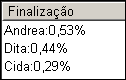
\includegraphics[scale=1.0]{./imagens/distribuicao_porcentagem.png}}
	\caption[Distribuição em porcentagem]
	{Distribuição em porcentagem \textbf{Fonte:} Desenvolvido pelos autores}
	\label{fig:distribuicao_porcentagem}
\end{figure}

\begin{itemize}
	\item Primeiramente deveria ser feito a soma de todas as porcentagens distribuídas, logo: 
	\par \texttt{0,53 + 0,44 + 0,29 = 1,26};
	
	\item o segundo passo seria calcular quanto cada porcentagem equivale dentro do total, neste 
	sentido o cálculo, já fazendo o arredondamento, seria: 
	\par \texttt{0,53 / 1,26 = 0,42 | 0,44 / 1,26 = 0,35 | 0,29 / 1,26 = 0,23}
	\par Logo, neste caso a Andrea seria responsável por 42\%, a Dita por 35\% e a Cida por 23\%;
	
	\item Assim, seria feito um cálculo com regra de 3 com o número total de peças. Supondo que o 
	 valor total fosse 500, logo:
	
	\par \texttt{(500 * 42) / 100 = 210 | (500 * 35) / 100 = 175 | (500 * 23) / 100 = 115}
	
	\par Neste caso então, a Andrea deveria produzir 210 peças, a Dita 175 e a Cida 115 peças;
	
	\item Por fim deveria ser feito uma divisão dos número de peças de cada costureira pela quantidade
     de peças por lote, que neste caso poderia ser 50, então realizando o cálculo já com arrendondamento:
     \par \texttt{210 / 50 = 4 | 175 / 50 = 4 | 115 / 50 = 2}
     
     \par Assim, a Andrea produziria 4 lotes, a Dita 4 e a Cida 2, dando o total
     dos 10 lotes a serem produzidos para a atividade de finalização.
	
\end{itemize}
 
 \par Os passos acima para distribuição de atividades seriam então repetidos
 para cada atividade chave do \texttt{HashMap} realizando tal distribuição para cada costureira da lista de 
 costureiras de cada atividade. No momento de fazer o último cálculo, foi feito
 um arredondamento, com isso se uma costureira tivesse tido uma porcentagem muito pequena, o valor de lotes para
 esta seria 0, eliminando-a assim da distribuição.
 
 \par Todavia verificou-se que, distribuindo desta forma, em alguns casos, o total de lotes por atividade não era distribuído
 de forma correta. Devido ao arredondamento, as vezes uma atividade ficava com lotes a menos ou lotes a mais do que o total
 definido, o que poderia causar erros no cálculo final. Além disso, no momento de definir como seria o cruzamento 
 surgiu uma questão importante que é o fato de que todas as vezes que fosse criado um indivíduo a partir de outros, deveria
 ser realizado o cálculo de normalização, e com isso a distribuição de lotes no novo indivíduo poderia ficar completamente
 diferente de seus pais, resultando assim na quebra do paradigma de algoritmos genéticos que descreve que os indivíduos filhos
 devem ser formados pela mesclagem das características dos pais. 


\par Buscou-se então uma outra alternativa para se realizar a distribuição dos lotes e definiu-se que, ao invés de distribuir
a porcentagem, a distribuição já deveria ser feita a nível de lote sendo esta também realizada de forma aleatória. Os parâmetros
do \texttt{construtor} da classe \texttt{ProcessoIndividuo} permaneceram da mesma forma, alternando somente a forma com que 
os lotes são distribuídos entre as costureiras em cada atividade conforme mostra
o Código ~\ref{fig:distribuicaoDiretamente}.


\begin{lstlisting} [style=custom_Java,caption={[Métodos da classe \texttt{FilmeBean}]{Distribuição em lotes diretamente. \textbf{Fonte:} Elaborado pelos autores.}}, label=fig:distribuicaoDiretamente] 	

public ProcessoIndividual(Atividade atividadeFinal,
	BigDecimal prazoEmSegundos, 
	Map<Integer, List<CostureiraHabilidade>> atividadesCostureiras, 
	int numeroLote, int pecasPorLote){
	
	chromosomes = new ArrayList<Chromosome>();
	Map<Integer, ProcessoChromosome> chromossomosMap = 
		new HashMap<Integer, ProcessoChromosome>();
	
	this.atividadeFinal = atividadeFinal;
	this.numeroLote = numeroLote;
	this.pecasPorLote = pecasPorLote;
	this.prazo = prazoEmSegundos;
	
	boolean distribuiuPorTodasCostureiras = false;
	
	int qtdeLote = 0;
	int cont = 0;
	
	for (Integer key : atividadesCostureiras.keySet()) {
		qtdeLote = numeroLote;
		cont = 0;
		int loteCostureira = 0;
		distribuiuPorTodasCostureiras = false;
		
		while (true){
			/* Verificou-se que quando a qtdeLote era 1 o valor
			   sorteado nunca era zero usando o Math.random com 
			   CAST para INT */
			if(qtdeLote == 1){
				loteCostureira  = Math.round((float) Math.random() * 1);
			}else{
				loteCostureira = (int) (Math.random() * qtdeLote);
			}
		
			CostureiraHabilidade costureiraHabilidade = 
				atividadesCostureiras.get(key).get(cont);
				
			ProcessoChromosome intermediario = 
				chromossomosMap.get(costureiraHabilidade.getIdCostureiraHabilidade());
				
			if(intermediario == null){
				ProcessoChromosome pc = new ProcessoChromosome
					(key, costureiraHabilidade,loteCostureira); 
					
				chromossomosMap.put
					(costureiraHabilidade.getIdCostureiraHabilidade(), pc);
					
				chromosomes.add(pc);
			}else{
				int oldValue = intermediario.getQuantidade_lotes();
				int newValue = oldValue + loteCostureira;
				intermediario.setQuantidade_lotes(newValue);
				intermediario.setLotesToShow(newValue);
			}
			
			if (cont == atividadesCostureiras.get(key).size() - 1) {
				cont = -1;
				distribuiuPorTodasCostureiras = true;
			} 
	
			qtdeLote -= loteCostureira;
			
			if(qtdeLote == 0 && distribuiuPorTodasCostureiras){
				break;
			}
			cont++;
		}
	}
}

\end{lstlisting}
 
\par Conforme descrito no Código ~\ref{fig:distribuicaoDiretamente}, é feita uma
iteração no \texttt{HashMap} e, para cada atividade, é feita a distribuição dos lotes para
as costureiras desta lista. O algoritmo então atribui a cada costureira um valor
que pode variar de 0 até \texttt{qtdeLote}. Assim é criado objetos da classe \texttt{ProcessoChromosome} 
e colocado na lista de cromossomos do indivíduo. Após a criação de cada cromossomo, a quantidade de
lotes é subtraída pelo valor atribuído ao cromossomo recém criado.
Se a iteração passar por todas as costureiras da lista, o contador é reiniciado e então, se ao final sobrar 
lotes a serem distribuídos, a distribuição recomeça na primeira costureira, acrescentando assim seu 
número de lotes de acordo com o novo valor sorteado. A iteração termina quando não há mais lotes a serem 
distribuídos e a execução já passou por todas as costureiras. Em uma primeira versão, quando a execução chegava
ao final da lista de costureiras e ainda existiam lotes a serem distribuídos, este restante de lotes era atribuído
à última costureira, porém verificou-se, que desta forma, o algoritmo tendia a nunca distribuir zero lotes à última
costureira, o que causou resultados ineficazes na distribuição. Alterando para esta forma, a distribuição  passou a 
ser feita de maneira totalmente uniforme deixando o resultado coerente.
Como é possível perceber, neste processo uma costureira pode receber aleatoriamente o valor 0, o que irá resultar na 
sua eliminação do processo da mesma forma que iria ocorrer na primeira abordagem. Por fim, após a finalização do primeiro
\texttt{for} um novo indivíduo terá sido criado, semelhante ao quadro
apresentado na Figura ~\ref{fig:distribuicao_lotes_costureiras}.

\par Concluindo, a distribuição das atividades ocorre todas as vezes que se cria um novo indivíduo.
Tais indivíduos podem ser criados no processo de criação da \texttt{população inicial}, na criação de 
\texttt{indivíduos estrangeiros} e no processo de \texttt{cruzamento}, como será descrito nas próximas seções,
ressaltando porém que no processo de cruzamento, os cromossomos do indivíduo é a mistura dos cromossomos dos pais,
já criados anteriormente, e portanto há também um construtor na classe \texttt{ProcessoIndividual} que recebe uma lista de 
cromossomos para se criar um novo indivíduo. Este processo será demonstrado na seção que descreve o cruzamento.


\subsection{Função de avaliação}

\par Após a criação da população inicial, esta é então submetida a um processo
de avaliação. Assim é feita uma iteração sobre a lista de indivíduos e para cada um é chamado então o seu método 
\texttt{calculateValue()}. Tal método é declarado de forma abstrata na classe mãe
\texttt{Individual} e implementado na classe \texttt{ProcessoIndividual}.

\par Assim como já foi visto anteriormente, cada costureira sabe fazer uma ou
mais partes da calça e gasta um determinado tempo, medido em segundos, além de cobrar um valor 
para se produzir cada peça, que varia de  acordo com a habilidade, além disto, existe um 
tempo de transporte entre cada costureira que é medido através da distância euclidiana, 
ou seja, cada costureira recebe um valor X e Y que representam suas localidades e então, 
através da formula euclidiana, é possível calcular a distância entre elas. A Figura 
~\ref{fig:demonstracao_costureiras_habilidades} demonstra os dados a serem considerados para o
cálculo do valor do indivíduo.


\begin{figure}[h!]
	\centerline{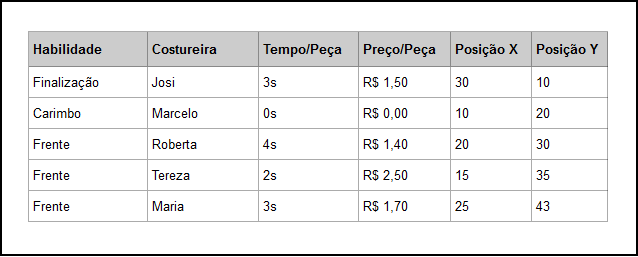
\includegraphics[scale=0.5]{./imagens/tempo_habilidade_3.PNG}}
	\caption[Demonstração de costureiras e habilidades]
	{Demonstração de costureiras e habilidades \textbf{Fonte:} Desenvolvido pelos
	autores.}
	\label{fig:demonstracao_costureiras_habilidades}
\end{figure}

\par Com base nestes dados é realizado um cálculo a fim de se encontrar o tempo total de fabricação do número de peças
desejado e, ao fim, um valor de tempo e custo de produção será atribuído ao indivíduo, tais valores serão utilizados 
posteriormente no processo de classificação.

\par Para o desenvolvimento do cálculo do tempo de produção, foi necessário construir uma estrutura para representar a 
questão da ordem de precedência entre as atividades. Tal estrutura, conforme é demonstrado na Figura ~\ref{fig:montagem_node}, 
deveria ter nós representando cada atividade, as costureiras que trabalham em cada atividade e o número de lotes atribuídos a 
cada uma aleatoriamente pelo algoritmo.

%\newpage

\begin{figure}[h!]
	\centerline{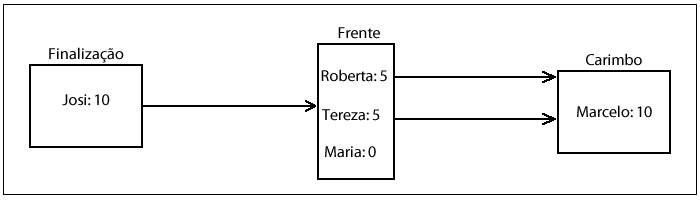
\includegraphics[scale=1.1]{./imagens/montagem_node.png}}
	\caption[Estrutura de representação da ordem de precedência]
	{Estrutura de representação da ordem de precedência \textbf{Fonte:}
	Desenvolvido pelos autores.}
	\label{fig:montagem_node}
\end{figure}


\par Como foi visto na seção 1.4.2, cada indivíduo possui uma lista de
cromossomos, e cada cromossomo, por sua vez, representa a alocação de uma
costureira, contendo os lotes que esta deve produzir para uma determinada atividade.
Desta forma, para calcular o custo total de produção, foi realizada uma iteração 
na lista de cromossomos do indivíduo somando o preço total de confecção dos lotes
que cada costureira recebeu aleatoriamente pelo algoritmo conforme mostra o Código
~\ref{list:metodoCalculateValue}.

\par Para o cálculo do tempo de produção, definiu-se então que tal lista de cromossomos deveria ser
dividida de forma que se pudesse agrupar os cromossomos por atividade estabelecendo assim a relação 
demonstrada na Figura ~\ref{fig:demonstracao_costureiras_habilidades}, para, que
por fim, o cálculo pudesse ser realizado.
Para isso, conforme demonstrado no Código ~\ref{list:metodoCalculateValue}, primeiramente, a lista de 
cromossomos foi distribuída em um \texttt{HashMap} denominado \texttt{atividadeCromossomos}, contendo 
como chave a atividade e como valor a lista de cromossomos para a respectiva atividade e foi criado uma 
classe denominada \texttt{Node}, sendo esta a responsável por criar a estrutura
mostrada na Figura ~\ref{fig:demonstracao_costureiras_habilidades}.

\par O método \texttt{calculateValue()}, após agrupar os cromossomos por atividade, 
 instancia um objeto da classe \texttt{Node} passando a \texttt{atividadeFinal} e o número de 
 peças por lote recebidos na criação do indivíduo, conforme descrito na seção anterior, e o map 
 atividadeCromossomos conforme mostra a Código ~\ref{list:metodoCalculateValue}.


\begin{lstlisting} [style=custom_Java,caption={[Métodos da classe \texttt{FilmeBean}]{Método \texttt{calculateValue()}. \textbf{Fonte:} Elaborado pelos autores.}}, label=list:metodoCalculateValue] 	

	public void calculateValue() {
		Map<Integer, List<Chromosome>> atividadeCromossomos 
			= new HashMap<Integer, List<Chromosome>>();
		
		Integer lastAtividade = null;
		float custoTotal = 0;
		int totalPecasAProduzir = 0;
		List<Chromosome> cromossomos = null;
		
		/*Calcular o custo total*/
		for(Chromosome chromosomeCusto : chromosomes){
			totalPecasAProduzir = 0;
			ProcessoChromosome processoChromossome = 
				(ProcessoChromosome) chromosomeCusto;
				
			totalPecasAProduzir = 
				processoChromossome.getLotesToShow() * this.pecasPorLote;
				
			custoTotal += totalPecasAProduzir * 
				processoChromossome.getCostureiraHabilidade()
					.getPrecoPorPeca();
		}
		
		for (Chromosome chromosome : chromosomes) {
		ProcessoChromosome processoChromossome = (ProcessoChromosome) chromosome;
		
			if (lastAtividade == null || lastAtividade != processoChromossome.getAtividade()) {
				cromossomos = new ArrayList<Chromosome>();
				
				atividadeCromossomos.put
					(processoChromossome.getAtividade(),cromossomos);
				lastAtividade = processoChromossome.getAtividade();
			}
			cromossomos.add(processoChromossome);
		}
		node = new Node(atividadeFinal, atividadeCromossomos,this.pecasPorLote);
		
		setCusto(custoTotal);
		
		
		/*So deve-se calcular o valor do individuo se 
		  ele nao foi calculado ainda porque uma vez calculado 
		  o valor o numero de lotes no objeto cromossomo foi 
		  decrementado */
		if (getValue() == 0) {
			setValue(node.getValorTotal());
			setRootNode(node);
		}
	}

\end{lstlisting}


\par A estrutura da classe \texttt{Node} foi realizada de forma a produzir objetos de si mesma de forma recursiva, assim 
cada vez que esta é instanciada, é como se criasse um nó daqueles
mostrados na Figura ~\ref{fig:demonstracao_costureiras_habilidades}. Assim,
quando o método \texttt{calculateValue()} instancia um objeto \texttt{Node}, no construtor deste outros nós são criados, e então toda
estrutura, como foi ilustrada na Figura
~\ref{fig:demonstracao_costureiras_habilidades}, será criada. O Código
~\ref{list:classeNode} mostra a construção de um objeto \texttt{Node}.

\begin{lstlisting} [style=custom_Java,caption={[Métodos da classe
\texttt{FilmeBean}]{Construtor da classe Node. \textbf{Fonte:} Elaborado pelos
autores.}}, label=list:classeNode]

	public Node(Atividade atividade,Map<Integer,List<Chromosome>>
		 atividadeCromossomos, int pecasPorLote){
		
		this.atividade = atividade;
		this.pecasPorLote = pecasPorLote;
		cromossomos = atividadeCromossomos.
			get(atividade.getIdAtividade());
			
		Atividade atividadePredecessora = null;
		
		for(AtividadeOrdem predecessora : 
			atividade.getAtividadeOrdemsForIdAtividade()){
			
			atividadePredecessora = 
				predecessora.getAtividadePredecessora();
		
			predecesoras.add(new Node(atividadePredecessora,
				atividadeCromossomos,pecasPorLote));
		}
	}
\end{lstlisting}

\par A classe \texttt{Node} recebe em seu construtor um objeto de Atividade, que na primeira vez que o objeto for instanciado
será a atividade final, o \texttt{MAP} com todos os cromossomos e o número de peças por lote, que será utilizado posteriormente.
O construtor então armazena as informações e pega do \texttt{MAP} somente os cromossomos relacionados a atividade recebida e, 
por fim, faz uma iteração na lista de atividades predecessoras da atividade recebida e, recursivamente, cria novos nós, 
construindo assim, a estrutura demonstrada na Figura
~\ref{fig:demonstracao_costureiras_habilidades}.

\par Como se pode ver no método \texttt{calculateValue()} no Código
~\ref{list:metodoCalculateValue}, após criar a estrutura de nós, é chamado o método \texttt{getValorTotal()} do objeto
\texttt{node} criado. Este método é responsável por iniciar a sequência lógica que 
faz o cálculo do tempo total a ser gasto pelo indivíduo, calculando o tempo gasto por 
cada costureira, definindo quem irá enviar peças pra quem e calculando o tempo de transporte 
de cada envio, conforme demonstra Código ~\ref{list:codigo_metodo_get_valor_total} .

\begin{lstlisting} [style=custom_Java,caption={[Método \texttt{getValorTotal()}]{Método \texttt{getValorTotal()}. \textbf{Fonte:} Elaborado pelos autores.}}, label=list:codigo_metodo_get_valor_total] 	

	public long getValorTotal(){
		long valor =  0;
		long maior = 0;
		
		for(Chromosome chromosome : cromossomos){
			ProcessoChromosome processoChromosome = 
				(ProcessoChromosome) chromosome;
		
			if(processoChromosome.getQuantidade_lotes() > 0){
				valor = getCromossomeValue(processoChromosome,
					processoChromosome.getQuantidade_lotes());
			}
	
			if(valor > maior){
				maior = valor;
			}
		}
		return maior;
	}

\end{lstlisting}


\par O método faz uma iteração na lista de cromossomos do nó da atividade final e irá chamar o método getChromosomeValue passando 
cada cromossomo e o valor de seus lotes, e irá retornar o valor do maior cromossomo.

\par Tomando como base a Figura ~\ref{fig:montagem_node}, para facilitar o
entendimento, o método getChromosomeValue() será chamado passando o cromossomo "Josi" e o inteiro 10 na quantidade de lotes. 
Este método é responsável por calcular o tempo gasto 
pela costureira para realizar os lotes atribuídos a ela. O tempo gasto pela
costureira é definido por \texttt{NLC * QPL * TP}, onde: \texttt{NLC} é o número
de lotes atribuídos para a costureira, \texttt{QPL} é a quantidade de peças por
lote e o \texttt{TP} é o tempo que a costureira gasta para fazer cada peça, 
porém este tempo também é influenciado pelo tempo que se é gasto para receber 
as partes dependentes, conforme demonstra o código ~\ref{list:codigo_metodo_get_cromossome_value}.


\begin{lstlisting} [style=custom_Java,caption={[Método \texttt{getValorTotal()}]{Método \texttt{getCromossomeValue()}. \textbf{Fonte:} Elaborado pelos autores.}}, label=list:codigo_metodo_get_cromossome_value] 	

public long getCromossomeValue(ProcessoChromosome processoChromosome,
	int qtdeLote){
	
	long valor = 0;
	valor = qtdeLote * this.pecasPorLote *
		 processoChromosome.getCostureiraHabilidade().getTempoPorPeca();

	valor += getTempoRecebimentoPecas(processoChromosome,qtdeLote);
	return valor;
}

\end{lstlisting}

\par O método \texttt{getChromossomeValue()} chama então o método getTempoRecebimentoPecas(), passando o cromossomo Josi e 
o inteiro 10 como quantidade de lote. O método chamado tem a função de fazer uma busca nos nós predecessores buscando encontrar 
qual o tempo gasto para o recebimento das partes predecessoras da atividade e retornar o maior valor, 
conforme demonstra o Código ~\ref{list:codigo_metodo_get_recebimento_pecas}.

\begin{lstlisting} [style=custom_Java,caption={[Método \texttt{getValorTotal()}]{Método \texttt{getTempoRecebimentoPecas()}. \textbf{Fonte:} Elaborado pelos autores.}}, label=list:codigo_metodo_get_recebimento_pecas] 	

	public long getTempoRecebimentoPecas(
		ProcessoChromosome processoChromosome, int qtdeLote){
		
		long valor = 0;
		long maior = 0;
		
		for(Node node : predecesoras){
			valor = node.getValueChromosomosPredecessores(
				processoChromosome, qtdeLote);
			
			if(valor > maior){
				maior = valor;
			}
		}
		return maior;
	}
}

\end{lstlisting}


\par Neste ponto começa então um processo recursivo, pois é chamado um método da
própria classe Node, só que de uma outra instância. O método chamado é o getValueChromosomosPredecessores() 
passando o cromossomo Josi e o inteiro 10, como número de lotes. O código ~\ref{list:codigo_metodo_getValueChromosomosPredecessores} 
mostra este método.


\begin{lstlisting} [style=custom_Java,caption={[Método \texttt{getValorTotal()}]{Método \texttt{getValueChromosomosPredecessores()}. \textbf{Fonte:} Elaborado pelos autores.}}, label=list:codigo_metodo_getValueChromosomosPredecessores] 	

	public long getValueChromosomosPredecessores(
		ProcessoChromosome processoChromosome,int qtdeLote){
	
		int qtdeEachCromossome = 0;
		long valor = 0;
		long maior = 0;
		long distance = 0;
		
		for(Chromosome chromosome : cromossomos){
			ProcessoChromosome processoChromosomeBefore =
			   (ProcessoChromosome) chromosome;
			
			qtdeEachCromossome =
			   processoChromosomeBefore.getQtdeLotes(qtdeLote);
			
			if(qtdeEachCromossome > 0){
				qtdeLote -= qtdeEachCromossome;
				valor = getCromossomeValue(
					processoChromosomeBefore, qtdeEachCromossome);
					
				distance = calcularTempoEntreCostureiras(
					processoChromosome, processoChromosomeBefore);
				
				processoChromosome.addCostureiraPredecessora(
					processoChromosomeBefore.getCostureiraHabilidade(), 
					
				qtdeEachCromossome,distance,valor);
				
				valor += distance;
			}
			
			if(valor > maior){
				maior = valor;
			}
			
			if(qtdeLote == 0){
				break;
			}
		}
		return maior;
	}	
\end{lstlisting}

\par Tal método é responsável por iterar sobre a lista de cromossomos do nó anterior buscando de qual ou quais costureiras 
podem ser obtidos os lotes, retornando o maior valor. No exemplo da Figura ~\ref{fig:ex_solicitaca_lotes}, a atividade anterior é a ``Frente'' e a primeira costureira da lista é a Roberta, neste caso a Josi solicita 10 lotes da parte da frente para a Roberta, porém, 
neste caso, a Roberta confeccionou somente 5 lotes, neste caso , a Josi irá consumir os 5 lotes confeccionados.


\begin{figure}[h!]
	\centerline{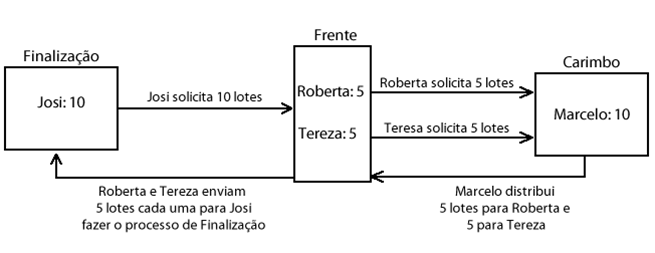
\includegraphics[scale=1.2]{./imagens/distribuicao_exemplo_apresentacao.png}}
	\caption[Exemplo de solicitação de lotes predecessores]
	{Exemplo de solicitação de lotes predecessores
	\textbf{Fonte:} Desenvolvido pelos autores.}
	\label{fig:ex_solicitaca_lotes}
\end{figure}


\par Assim, a costureira Roberta é adicionada ao cromossomo Josi como costureira predecessora e novamente é chamado o método \texttt{getChromosomeValue()}, só que agora passando o cromossomo Roberta e a quantidade de lote que ela deve produzir para 
atender a Josi, para que se possa calcular o tempo, além disso será chamado o método calcularTempoEntreCostureiras() que irá 
retornar o tempo de transporte entre a Josi e a Roberta, e será somado ao valor retornado de \texttt{getChromosomeValue()} que  
foi chamado passando o cromossomo Roberta. O Código ~\ref{list:codigo_metodo_calcularTempoEntreCostureiras} demonstra este método \texttt{calcularTempoEntreCostureiras()}.



\begin{lstlisting} [style=custom_Java,caption={[Método \texttt{getValorTotal()}]{Método \texttt{getValueChromosomosPredecessores()}. \textbf{Fonte:} Elaborado pelos autores.}}, label=list:codigo_metodo_calcularTempoEntreCostureiras] 	

	public long calcularTempoEntreCostureiras(
		ProcessoChromosome processoChromosome,
		ProcessoChromosome processoChromosomeBefore){
		
		int posicaoCostureiraX = processoChromosome.
			getCostureiraHabilidade().
			getCostureira().getPositionX();
			
		int posicaoCostureiraY = processoChromosome.
			getCostureiraHabilidade().
			getCostureira().getPositionY();
		
		int posicaoCostureiraBeforeX = processoChromosomeBefore.
			getCostureiraHabilidade().
			getCostureira().getPositionX();
			
		int posicaoCostureiraBeforeY = processoChromosomeBefore.
			getCostureiraHabilidade().
			getCostureira().getPositionY();
		
		long distance = (long) Math.sqrt(
		Math.pow(posicaoCostureiraX - posicaoCostureiraBeforeX, 2)+
		Math.pow(posicaoCostureiraY - posicaoCostureiraBeforeY, 2));
		
		return distance * 100;
	}

\end{lstlisting}

\par Seguindo as execuções dos métodos já explicados, o fluxo de chamadas então será \texttt{getCromossomeValue()}, \texttt{getTempoRecebimentoPecas()}, getValueChromosomosPredecessores() e neste ponto o cromossomo Roberta irá solicitar 
para sua atividade anterior, 5 lotes, conforme mostra a Figura ~\ref{fig:ex_solicitaca_lotes}.

\par Neste caso, a atividade anterior é o Carimbo, neste ponto existe uma exceção, pois quando 
se solicita para atividade Carimbo, não são consumidos os lotes desta, pois, conforme definido 
no escopo explicado anteriormente, a atividade de Carimbo só possui o Marcelo como trabalhador e ele
apenas distribui o material de costura, assim qualquer solicitação feita a ele é correspondida, além 
disso como o tempo de produção e o custo por peça do Marcelo é zero, só sera considerado apenas
o tempo de transporte entre o Marcelo e a Roberta.

\par E assim, todo  o processo é feito recursivamente, na qual as costureiras
da primeira atividade vão consumindo os lotes das costureiras das atividades
predecessoras, conforme mostra a Figura ~\ref{fig:ex_solicitaca_lotes}.
Como a Roberta não conseguiu atender a Josi, uma vez calculado o tempo de produção ds 5 peças da Roberta, 
o algoritmo verifica a próxima costureira da atividade Frente, que seria a Tereza neste exemplo, e, da mesma forma, calcula
o tempo de produção do número de peças solicitadas que seria 5 neste caso.

\par Concluindo, o processo é todo feito recursivamente, na qual as costureiras das primeiras atividades vão consumindo
os lotes das costureiras das atividades predecessoras e somado o tempo de produção e o tempo de transporte entre elas, 
conforme mostra a Figura ~\ref{fig:ex_tempo_producao}. 


\begin{figure}[h!]
	\centerline{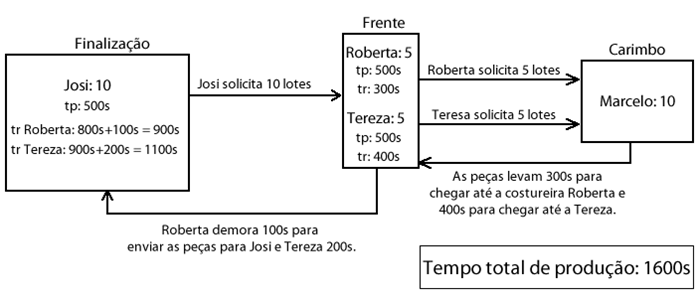
\includegraphics[scale=1.2]{./imagens/distribuicao_tempo.png}}
	\caption[Distribuição demonstrando o tempo]
	{Distribuição demonstrando o tempo
		\textbf{Fonte:} Desenvolvido pelos autores.}
	\label{fig:ex_tempo_producao}
\end{figure}

A recursividade para quando se chega na atividade Carimbo, então os valores começam a ser retornados.  No fim, prevalece sempre o 
maior valor e assim o método \texttt{getValorTotal()} irá retornar o tempo total de produção das partes e o transporte das mesmas 
entre as costureiras e então este valor é colocado no atributo \texttt{value} do indivíduo.

\par A função de avaliação é chamada dentro do método \texttt{classify}, dentro da classe \texttt{GAController}, tal método, 
por sua vez, é chamado dentro do método \texttt{execute()} após a criação da população inicial.

\subsection{Classificação dos indivíduos}
\par Uma vez definido os valores de tempo total de produção e custo do indivíduo, o próximo passo a ser realizado, dentro da
ordem de execução do algoritmo genético, é a classificação dos indivíduos. Tal classificação também é realizada no método 
\texttt{classify} da classe \texttt{GAController}, conforme mostra o Código ~\ref{list:codigo_metodo_classify}.


\begin{lstlisting} [style=custom_Java,caption={[Método \texttt{classify()}]{Método \texttt{classify()}. \textbf{Fonte:} Elaborado pelos autores.}}, label=list:codigo_metodo_classify] 

public void classify(List<Individual> population){
	List<Individual> populationAux = new ArrayList<Individual>();
	List<Individual> populationGood = new ArrayList<Individual>();
	
	for(Individual individual : population){
		individual.calculateValue();
	}
	Collections.sort(population);
		
		
	for(Individual individual : population){
			
		ProcessoIndividual pi = (ProcessoIndividual) individual;
		if(individual.getValue() <= pi.getPrazo().longValue()){
			individual.setTipoDeClassificacao(
				Constants.CLASSIFICACAO_POR_CUSTO);
				
			populationGood.add(individual);
		}
	}
	Collections.sort(populationGood);
				
	for(Individual individual : populationGood){
		individual.setTipoDeClassificacao(
			Constants.CLASSIFICACAO_POR_TEMPO);
	}
					
	//Remove todos os objetos com tempo < prazo da populacao
	population.removeAll(populationGood);
				
	//Adiciona-os na populacao auxiliar
	populationAux.addAll(populationGood);
					
	//adiciona os demais individuos da populacao
	populationAux.addAll(population);
				
	//Redefine a populacaoo
	population.clear();
	population.addAll(populationAux);
					
}
						
\end{lstlisting}

\par Após chamar a função de avaliação para todos os indivíduos, através do método \texttt{calculateValue()}, o método
de ordenação \texttt{Collections.sort()} é chamado passando a lista de indivíduos (população). Para que se possa utilizar este método
de ordenação, a classe, que representa o tipo da lista, deve implementar a interface
\texttt{Comparable} e, ao implementá-la, obrigatoriamente o método \texttt{compareTo()} deve ser implementado. Este método
define qual será o critério de comparação durante a ordenação da lista. No caso do método \texttt{compareTo} da classe Individual, 
implementado na classe \texttt{ProcessoIndividual}, por ter sido declarado como abstrato, foi definido uma \textit{flag} de forma a
definir se os indivíduos devem ser ordenados pelo tempo total ou pelo custo, conforme mostra o Código ~\ref{list:codigo_metodo_compareTo}.

\begin{lstlisting} [style=custom_Java,caption={[Método \texttt{compareTo()}]{Método \texttt{compareTo()}. \textbf{Fonte:} Elaborado pelos autores.}}, label=list:codigo_metodo_compareTo] 

	@Override
	public int compareTo(Individual o) {
		if(tipoDeClassificacao == Constants.CLASSIFICACAO_POR_CUSTO){
			return Float.compare(getCusto(), o.getCusto());
		}else{
			return Float.compare(getTempo(), o.getTempo());
		}
	}

\end{lstlisting}

\par O atributo \texttt{tipoDeClassificacao} é iniciado com zero, ou seja, o padrão é que a classificação seja realizada levando 
em consideração o tempo total de produção de cada indivíduo. Desta forma, no Código  ~\ref{list:codigo_metodo_classify}, na linha
9, a ordenação da população será com base no tempo de produção. A questão é que, de acordo com o escopo definido, o objetivo do 
algoritmo seria encontrar um baixo tempo de produção associado a um custo minimizado, de forma que a melhor solução fosse aquela
que permitisse a produção das calças no menor custo com um tempo menor ou igual ao prazo, este prazo foi passado pelo usuário e
atribuído ao indivíduo no construtor da classe \texttt{ProcessoIndivíduo}, conforme já explicado na seção anterior. 

\par Desta forma, de acordo com o Código ~\ref{list:codigo_metodo_classify}, após a ordenação da população pelo tempo de produção, 
é feita uma verificação para buscar todos os indivíduos que possuem tempo de produção menor ou igual ao prazo e, os indivíduos que antedem este requisito, recebem o valor 1 no atributo \texttt{tipoDeClassificacao}(ordenação por custo), alem disto são adicionados a uma outra lista denominada \texttt{populationGood}, que também será ordenada, só que agora o critério de ordenação do método \texttt{compareTo()} passou ser o custo. Após esta ordenação o atributo \texttt{tipoDeClassificacao} é zerado para evitar possíveis inconsistência em futuras ordenações e, com ajuda de listas auxiliares, os objetos da lista \texttt{populationGood} são transferidos para as primeiras posições da população e os demais indivíduos acrescentados ao final.

\par Desta forma, o algoritmo irá manter sempre o menor custo, procurando manter o tempo dentro do prazo, porém caso nenhum dos indivíduos tenham o tempo total menor que o prazo, então o melhor tempo é retornado e a ordenação por custo é ignorada.

\subsection{Indivíduos estrangeiros e elitismo}

\par Após a classificação dos indivíduos, o próximo passo, a ser realizado pelo método \texttt{execute()}, é verificar
se o melhor indivíduo (primeiro da lista) da população atual é melhor que o da população anterior, caso positivo ou
caso a população atual seja a população inicial a variável \texttt{lastBest} recebe este melhor indivíduo e então é 
realizada uma verificação para checar se o número de gerações (atributo \texttt{getGenerationQuantity}) foi atingido, 
caso positivo a execução é interrompida e o indivíduo armazenado na variável \texttt{lastBest} é retornado, ao contrário, 
a execução irá continuar de forma a iniciar a criação de uma nova população conforme mostra o Código ~\ref{list:código_metodo_execute}.

\newpage

\begin{lstlisting} [style=custom_Java,caption={[Método \texttt{execute()}]{Método \texttt{execute()}. \textbf{Fonte:} Elaborado pelos autores.}}, label=list:código_metodo_execute] 

	public Individual execute(){
		model.createInitialPopulation();
		Individual lastBest = null;
		
		for(int i = 0; ; i++){
			ArrayList<Individual> population = model.getPopulation();
			ArrayList<Individual> newGeneration = 
				new ArrayList<Individual>();
			
			classify(population);
			if(lastBest == null || lastBest != population.get(0)){
				lastBest = population.get(0);
			}
			
			//verifica o final da execucao
			if(i == model.getGenerationQuantity()){
				break;
			}
			
			//A partir deste ponto e iniciado a criacao de 
			//uma nova populacao
			
			//elitismo
			if(model.isElitism()){
				doElistim(newGeneration);
			}
			
			int foreignQuantity = Math.round(
				model.getPopulationSize() * model.getForeignIndividualRate());
			
			foreignQuantity = foreignQuantity % 2 == 0 ? 
				foreignQuantity : foreignQuantity +1;
			
			for(int j = 0;j < foreignQuantity;j++ ){
				newGeneration.add(model.createIndividual());
			}
			
			while(newGeneration.size() < model.getPopulationSize()){
				//selecao
				Individual individual1 = doSelection();
				Individual individual2;
				
				do{
					individual2 = doSelection();
				}while(individual1 == individual2);
				
				//cruzamento
				IndividualPair pair = doCrossing(individual1, individual2);
				
				//mutacao
				doMutation(pair.getIndividual1());
				doMutation(pair.getIndividual2());
				
				newGeneration.add(pair.getIndividual1());
				newGeneration.add(pair.getIndividual2());
			}
			
			model.setPopulation(newGeneration);
		}
		return lastBest;
	}

\end{lstlisting}

\par O processo de criação de uma nova população inicia-se com o processo de elitismo. Tal processo, conforme já explicado
anteriormente, consiste em adicionar à nova população os dois melhores indivíduos da população anterior. O próximo
passo a ser executado é referente a adição de indivíduos à nova população, seguindo um conceito, existente no \textit{framework} de desenvolvimento adotado, denominado indivíduos estrangeiros. Este conceito considera o fato de que, na natureza, durante o processo de geração de uma nova população, indivíduos estrangeiros podem começar a fazer parte de tal população. 

\par No algoritmo genético, tais indivíduos simplesmente são introduzidos à nova população de acordo com uma taxa definida no 
atributo \texttt{foreignIndividualRate} da classe GAModel do \textit{framework}, conforme já explicado anteriormente. Conforme 
demonstrado na linha 36 do Código ~\ref{list:código_metodo_execute}, os indivíduos estrangeiros são criados utilizando o método \texttt{createIndividual()} da classe \texttt{GAModel} que foi implementado na classe \texttt{ProcessoModel}, 
tal método utiliza o mesmo construtor utilizado para criação de indivíduos da população inicial portanto segue a mesma lógica utilizada, a diferença é que, ao criar tais indivíduos, o \textit{looping} é executado de acordo com a taxa definida, o que irá resultar na criação de um número bem menor de indivíduos.

\subsection{Seleção de indivíduos e cruzamento} 

\par Após o processo de elitismo e a criação dos indivíduos estrangeiros, o restante da nova população é criado através do processo
de cruzamento, conforme as instruções a partir da linha 39 do Código ~\ref{list:código_metodo_execute}. O cruzamento começa com a 
seleção dos indivíduos que devem participar deste processo, esta seleção é realizada por meio do método \texttt{doSelection()} 
mostrado no Código ~\ref{list:metodoDoSelection}.

\begin{lstlisting} [style=custom_Java,caption={[Método \texttt{doSelection()}]{Método \texttt{doSelection()}. \textbf{Fonte:} Elaborado pelos autores.}}, label=list:metodoDoSelection] 

private Individual doSelection() {
	switch (model.getSelectionType()) {
		case CLASSIFICATION : return doSelectionByClassification();
		case ROULETTE: return doSelectionByRoulette();
	}
	return null;
}

\end{lstlisting}

\par O método verifica o atributo de configuração \texttt{selectionType} e, neste caso, o valor de tal atributo é 
\textit{CLASSIFICATION}, conforme mostrado na configuração do algoritmo genético na classe \texttt{GeneticAlgorithmManagement}, 
explanada anteriormente, portanto o método chamado é o \texttt{doSelectionByClassification()}, conforme mostra o Código
~\ref{list:metodo_doSelectionByClassification}.

\begin{lstlisting} [style=custom_Java,caption={[Método \texttt{doSelectionByClassification()}]{Método \texttt{doSelectionByClassification()}. \textbf{Fonte:} Elaborado pelos autores.}}, label=list:metodo_doSelectionByClassification] 

	private Individual doSelectionByClassification() {
		int maxValue = 0;
		
		for(int i = 0; i< model.getPopulationSize(); i++){
			maxValue += (i + 1);
		}
		
		double index = Math.random() * maxValue;
		int cursor = 0;
		
		for(int i = 0; i < model.getPopulationSize(); i++){
			cursor += model.getPopulationSize() - 1;
			
			if(index <= cursor){
				return model.getPopulation().get(i);
			}
		}
		
		return null;
	}


\end{lstlisting}

\par Tal método é responsável pela seleção de um indivíduo para realização do cruzamento. Primeiramente
é realizado a soma dos índices da lista de indivíduos (population) realizando um \texttt{FOR} de 0 até
\texttt{populationSize}, parâmetro que armazena o tamanho da população, assim se o tamanho da população for
7, a soma seria 1+2+3+4+5+6+7, o que daria um total de 28. Feito esta soma, é sorteado então um número 
entre zero até a soma dos valores e então é realizado um novo \texttt{FOR} de 0 até \texttt{populationSize},
dentro deste é feita uma verificação, se o número sorteado for menor ou igual 
a ao \texttt{populationSize} (\texttt{cursor}), que neste caso é 7, então o indivíduo da posição \texttt{i} (zero) é escolhido, 
caso não seja, a variável cursor é incrementada como o valor do tamanho da população, que neste caso resultaria 
em 14 e assim a verificação é feita novamente até que o número sorteado seja menor ou igual ao cursor e, quando assim
o for, o indivíduo da posição \texttt{i} é retornado. A figura Figura ~\ref{fig:ex_selecao} ilustra este processo.

\newpage

\begin{figure}[h!]
	\centerline{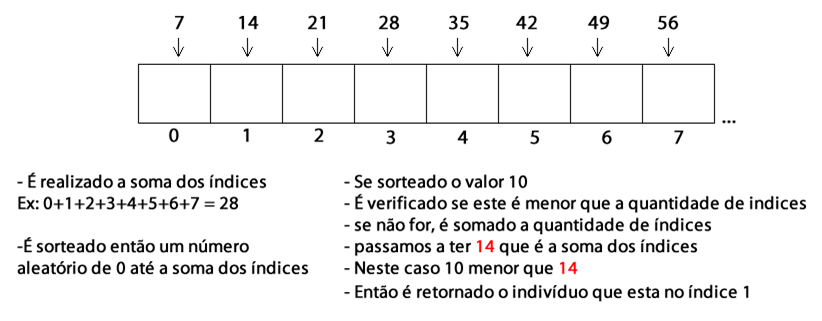
\includegraphics[scale=0.6]{./imagens/selecao.png}}
	\caption[Seleção dos indivíduos]
	{Representação do processo de seleção dos indivíduos
		\textbf{Fonte:} Desenvolvido pelos autores.}
	\label{fig:ex_selecao}
\end{figure}

\par Ao finalizar este processo um indivíduo terá sido escolhido, assim, de acordo com a linha 45 do Código ~\ref{list:código_metodo_execute},
um novo indivíduo deve ser selecionado, porém a instrução está dentro de um \texttt{do while} pois o processo deve ser repetido até que 
o novo indivíduo selecionado seja diferente do anterior evitando assim que dois indivíduos iguais façam parte do cruzamento.

\par O cruzamento é realizado a nível de cromossomos, neste caso, os indvíduos filhos recebem 
a mesclagem dos cromossomos de seus pais. No cruzamento desenvolvido para esta solução, foi 
necessário realizar um agrupamento dos cromossomos e então criar novos indivíduos através da
mesclagem destes grupos. Isto foi necessário pois, para cada atividade, o total de lotes,
distribuídos entre os cromossomos de cada atividade, não pode ser diferente do número total de lotes definido, assim o 
cruzamento então ocorre de forma que os indivíduos filhos recebem a mesclagem de grupos de 
cromossomos de seus pais referente a cada atividade e assim a cada cruzamento é criado
dois novos indivíduos que irão fazer parte da nova população. A Figura ~\ref{fig:ex_cruzamento} ilustra este processo.

\begin{figure}[h!]
	\centerline{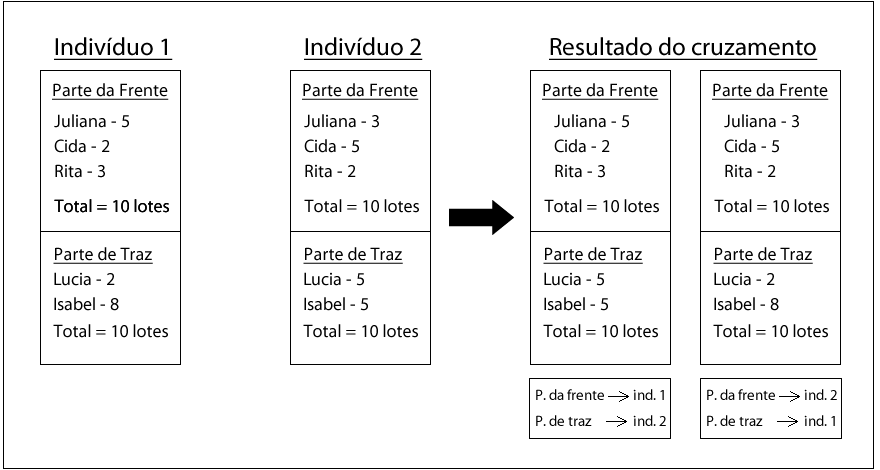
\includegraphics[scale=0.4]{./imagens/ex_cruzamento.png}}
	\caption[Cruzamento dos indivíduos]
	{Representação do processo de cruzamento dos indivíduos
		\textbf{Fonte:} Desenvolvido pelos autores.}
	\label{fig:ex_cruzamento}
\end{figure}


\par A partir da linha 49 do código Código ~\ref{list:código_metodo_execute}, dois indivíduos já foram selecionados e então o 
método \texttt{doCrossing()} é chamado para realizar o cruzamento. Tal método também verifica o tipo de cruzamento definido
chamando o método correspondente conforme mostra o Código ~\ref{list:metodoDoCrossing}. 



\begin{lstlisting} [style=custom_Java,caption={[Método \texttt{doCrossing()}]{Método \texttt{doCrossing()}. \textbf{Fonte:} Elaborado pelos autores.}}, label=list:metodoDoCrossing] 

	private IndividualPair doCrossing(Individual individual1, Individual individual2){
		switch (model.getCrossType()) {
			case ARITMETIC: break;
			
			case BINARY: 
				return doBinaryCrossing(individual1,individual2);
			case PERMUTATION: 
				return doPermutationCrossing(individual1, individual2);
		
			case UNIFORM:break;
		}
		return null;
	}

\end{lstlisting}


\par Neste caso, o método escolhido para o cruzamento foi o de permutação, desta forma o método \texttt{doPermutationCrossing()} é chamado.
Tal método faz parte do \texttt{framework} de desenvolvimento, porém foi modificado para se adaptar ao problema a ser resolvido pela 
aplicação conforme demonstrado no Código ~\ref{list:metodoPermutationCrossing}.


\begin{lstlisting} [style=custom_Java,caption={[Método \texttt{doPermutationCrossing()}]{Método \texttt{doPermutationCrossing()}. \textbf{Fonte:} Elaborado pelos autores.}}, label=list:metodoPermutationCrossing] 

		private IndividualPair doPermutationCrossing(
			Individual individual1, Individual individual2){
			
			ArrayList<Chromosome> chromosomes1 = 
				new ArrayList<Chromosome>();
				
			ArrayList<Chromosome> chromosomes2 = 
				new ArrayList<Chromosome>();
				
			Integer lastAtividade = null;
			float chooseIndividual = 0;
			int i = 0;
			
			for(Chromosome chromosome : individual1.getChromosomes()){
				ProcessoChromosome processoChromosome = 
					(ProcessoChromosome) chromosome;
				
				if(lastAtividade == null || 
					!lastAtividade.equals(processoChromosome.getAtividade())){
					
					chooseIndividual = Math.round((float) Math.random() * 1);
					lastAtividade = processoChromosome.getAtividade();
				}
				
				if(chooseIndividual == 1){
					chromosomes1.add(individual1.getChromosomes().
						get(i).clone());
						
					chromosomes2.add(individual2.getChromosomes().
						get(i).clone());
				}else{
					chromosomes1.add(individual2.getChromosomes().
						get(i).clone());
						
					chromosomes2.add(individual1.getChromosomes().
						get(i).clone());
				}
				i++;
			}
			
			Individual newIndividual1 = 
				model.createIndividual(chromosomes1);
				
			Individual newIndividual2 = 
				model.createIndividual(chromosomes2);
			
			return new IndividualPair(newIndividual1,newIndividual2);
		}
	

\end{lstlisting}

\par Conforme visto na Figura  ~\ref{fig:ex_cruzamento}, os cromossomos estão ordenados na lista de acordo com suas respectivas atividades, considerando isto, foi feita uma lógica para agrupar estes cromossomos por atividade e criar novos indivíduos através da mesclagem dos grupos criados de forma a sortear de qual indivíduo do cruzamento cada grupo deve ser pego ao criar um novo indivíduo. 

\par Assim, de acordo com o Código ~\ref{list:metodoPermutationCrossing}, primeiramente é feita uma iteração sobre a lista de cromossomos do indivíduo 1, dentro de tal iteração, é realizada uma verificação para checar se um cromossomo é o primeiro da primeira atividade (\texttt{lastAtividade == null}) ou se é o primeiro de um determinada atividade de acordo com a ordem delas, caso uma destas condições for verdadeira, um valor binário é sorteado, se tal valor for um, o primeiro novo indivíduo que será criado terá os cromossomos, da atividade em questão, pegos do indivíduo 1 do cruzamento e o segundo novo indivíduo receberá os cromossomos, referentes a tal atividade, do indivíduo 2, caso o valor sorteado seja zero, o processo acontece de forma inversa. 

\par Assim a iteração continua até a lista de cromossomos dos novos indivíduos possuir todos os grupos de cromossomos referentes a todas as atividades e então, ao fim da iteração, dois novos indivíduos serão criados através do método \texttt{createIndividual}.

\par Quando se cria indivíduos a partir deste ponto, a classe \texttt{ProcessoModel} utiliza um outro construtor para criar o indivíduo, conforme mostra o Código ~\ref{list:metodoCreateIndividualCromossomos}


\begin{lstlisting} [style=custom_Java,caption={[Método \texttt{creatIndividual()} utilzando cromossomos]{Método \texttt{creatIndividual()} utilizando cromossomos. \textbf{Fonte:} Elaborado pelos autores.}}, label=list:metodoCreateIndividualCromossomos] 

	@Override
	public Individual createIndividual(ArrayList<Chromosome> chromosomes) {
		return new ProcessoIndividual(atividadeFinal, prazoEmSegundos, chromosomes,this.numeroLote,this.pecasPorLote);
	}

\end{lstlisting}

\par Neste caso são passados quase todos os parâmetros enviados durante a criação
da população inicial, a diferença é que, neste caso, o indivíduo será criado a partir 
dos cromossomos conforme mostra o Código ~\ref{list:construtorDeIndividuosComCromossomos}.

\begin{lstlisting} [style=custom_Java,caption={[Construtor de \texttt{ProcessoIndividual} utilizando cromossomos]{Construtor de \texttt{ProcessoIndividual} utilizando cromossomos. \textbf{Fonte:} Elaborado pelos autores.}}, label=list:construtorDeIndividuosComCromossomos] 

public ProcessoIndividual(Atividade atividadeInicial, 
						  BigDecimal prazoEmSegundos, 
						  ArrayList<Chromosome> chromosomes, 
						  int numeroLote, int pecasPorLote) {

	super(chromosomes);
	this.atividadeFinal = atividadeInicial;
	this.numeroLote = numeroLote;
	this.pecasPorLote = pecasPorLote;
	this.prazo = prazoEmSegundos;
}

\end{lstlisting}
\par Os cromossomos recebidos são inseridos na lista de cromossomos declarada na classe mãe (\texttt{Individual}), e os 
outros parâmetros são atribuídos aos seus respectivos atributos. No final do método \texttt{doPermutaionCrossing}, como no 
Java não é possível retornar dois valores, é criado um objeto da classe \texttt{IndividualPair}, passando os dois novos indivíduos, 
e então este objeto é retornado. Esta classe só possui dois atributos do tipo \texttt{Individual} e só é utilizada para retornar os dois 
novos indivíduos criados.

\subsection{Mutação}
\par O processo de mutação, conforme já explicado anteriormente, consiste em realizar uma pequena modificação entre os cromossomos
de um indivíduo. Esta modificação pode ser boa, melhorando o resultado do indivíduo ou ruim. No algoritmo genético desenvolvido, 
a mutação foi realizada trocando o número de lotes recebidos entre duas costureiras escolhidas aleatoriamente dentro de um grupo de cromossomos de cada atividade do indivíduo, conforme mostra a Figura ~\ref{fig:ex_mutacao}.


\begin{figure}[h!]
	\centerline{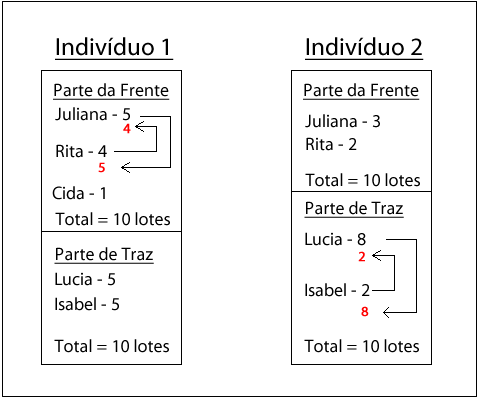
\includegraphics[scale=0.7]{./imagens/mutacao_cromossomo.png}}
	\caption[Exemplo de mutação]
	{Exemplo de mutação
		\textbf{Fonte:} Desenvolvido pelos autores.}
	\label{fig:ex_mutacao}
\end{figure}


\par O processo de mutação inicia-se dentro do método \texttt{execute()} da classe \texttt{GAController}, e é realizado nos indivíduos
criados, através do processo de cruzamento, dentro de uma determinada taxa, definida anteriormente nos atributos de configuração do algoritmo genético na classe \texttt{GeneticAlgorithmManagement}. O método que inicia este processo é o \texttt{doMutation()}, tal método verifica o tipo de mutação definido chamando o método correspondente, além disto, ele verifica se a mutação deve ser realizada, sorteando um número aleatoriamente e checando se o número sorteado é menor que a taxa de mutação definida, conforme mostra o Código ~\ref{list:metodoDoMutation}. 

\begin{lstlisting} [style=custom_Java,caption={[Método \texttt{doMutation()}]{Método \texttt{doMutation()}. \textbf{Fonte:} Elaborado pelos autores.}}, label=list:metodoDoMutation] 

	public void doMutation(Individual individual){
		if(Math.random() < model.getMutationRate()){
			for(int i = 0; i < model.getMutationQuantity();i++){
				switch (model.getMutation()) {
					case BINARY: doMutationBinary(individual);break;
					case NUMERICAL: break;
					case PERMUTATION: doMutationPermutation(individual);break;
				}
			}
		}
	}

\end{lstlisting}

\par Neste caso, o método escolhido para a mutação foi o de permutação, desta forma o método \texttt{doMutationPermutation()} é chamado.
Tal método faz parte do \texttt{framework} de desenvolvimento, porém também foi modificado para se adaptar ao problema a ser resolvido pela 
aplicação conforme demonstrado no Código ~\ref{list:metodoPermutationMutation}.


\begin{lstlisting} [style=custom_Java,caption={[Método \texttt{doMutationPermutation()}]{Método \texttt{doMutationPermutation()}. \textbf{Fonte:} Elaborado pelos autores.}}, label=list:metodoPermutationMutation] 

	public void doMutationPermutation(Individual individual) {
	
		Integer lastAtividade = null;
		ArrayList<ProcessoChromosome> chromossomesToMutate = 
			new ArrayList<ProcessoChromosome>(); 
		
		for(Chromosome chromosome : individual.getChromosomes()){
			ProcessoChromosome processoChromosome = 
				(ProcessoChromosome) chromosome;
			
			if(lastAtividade == null || 
				   !lastAtividade.equals(processoChromosome.getAtividade())){
				   
				if(!chromossomesToMutate.isEmpty() && 
					   chromossomesToMutate.size() > 1){
					
					doMutationOnChromossome(chromossomesToMutate);
				}
				chromossomesToMutate.clear();
				lastAtividade = processoChromosome.getAtividade();
			}
			chromossomesToMutate.add(processoChromosome);
		}
		//Para o ultimo grupo
		if(!chromossomesToMutate.isEmpty() && 
			   chromossomesToMutate.size() > 1){
			
			doMutationOnChromossome(chromossomesToMutate);
		}
	}

\end{lstlisting}

\par Para a realização da lógica que realiza a mutação, é realizada uma iteração na lista de cromossomos do 
indivíduo a qual a mutação será realizada, dentro desta iteração, os cromossomos de uma atividade são adicionados
à lista \texttt{chromossomesToMutate}, e assim, quando todos os cromossomos de uma atividade são adicionados nesta
lista, o método \texttt{doMutationOnCromossome} demonstrado no Código ~\ref{list:metododoMutationOnChromossome}, é
chamado para realizar a mutação, assim, após a mutação para os cromossomos de tal atividade, a lista \texttt{chromossomesToMutate} é zerada para que os cromossomos da próxima atividade sejam adicionados a esta e posteriormente sofram a mutação, logicamente, o grupo de atividades sofrerá mutação somente se possuir mais de um cromossomo.

\begin{lstlisting} [style=custom_Java,caption={[Método \texttt{doMutationOnChromossome()}]{Método \texttt{doMutationOnChromossome()}. \textbf{Fonte:} Elaborado pelos autores.}}, label=list:metododoMutationOnChromossome] 


	private void doMutationOnChromossome(
		ArrayList<ProcessoChromosome> chromossomesToMutate){
	
		int position1;
		int position2;
		int varAux;
		int varAux2;
		
		ProcessoChromosome chromosome1 = null;
		ProcessoChromosome chromosome2 = null;
		
		position1 = (int) (Math.random() * (chromossomesToMutate.size()));
		
		do{
			position2 = (int) (Math.random() * 
				(chromossomesToMutate.size()));
		}while(position1 == position2);
	
		chromosome1 = chromossomesToMutate.get(position1);
		chromosome2 = chromossomesToMutate.get(position2);
		
		varAux  = chromosome2.getQuantidade_lotes();
		varAux2 = chromosome2.getLotesToShow();
		
		chromosome2.setQuantidade_lotes(
			chromosome1.getQuantidade_lotes());
			
		chromosome2.setLotesToShow(chromosome1.getLotesToShow());
		
		chromosome1.setQuantidade_lotes(varAux);
		chromosome1.setLotesToShow(varAux2);
	}

\end{lstlisting}

\par Neste método, é selecionado quais cromossomos terão seus valores trocados entre si. O segundo cromossomo é escolhido dentro de um
\texttt{doWhile()} para evitar que o mesmo cromossomo escolhido na primeira vez seja selecionado e então, com auxilio de variáveis
auxiliares, os atributos \texttt{quantidade\_lotes} e \texttt{lotesToShow}, tem seus valores trocados entre si.

\subsection{Interface gráfica de distribuição} 

\par Para a interação do usuário com o algoritmo de distribuição e possibilidade de cadastro de cadastro de fluxos de processos e 
costureiras assim como suas respectivas habilidades, tempo e preço de produção, foi realizado uma aplicação em plataforma \texttt{web}
utilizando \textit{JSF} e \textit{Primefaces}, porém a forma que o mecanismo de cadastro das informações foi realizado não é relevante
ser apresentado mas é importante explanar sobre o desenvolvimento da tela de distribuição das atividades, a qual é de extrema importância para 
entender o fluxo de execução da aplicação. No menu "Distribuir tarefas" da aplicação estão disponíveis todos os processos cadastrados e
para abrir a tela de distribuição de atividades basta clicar no ícone "abrir" da coluna opções conforme mostra a Figura ~\ref{fig:tela_dis_processos}.

\begin{figure}[h!]
	\centerline{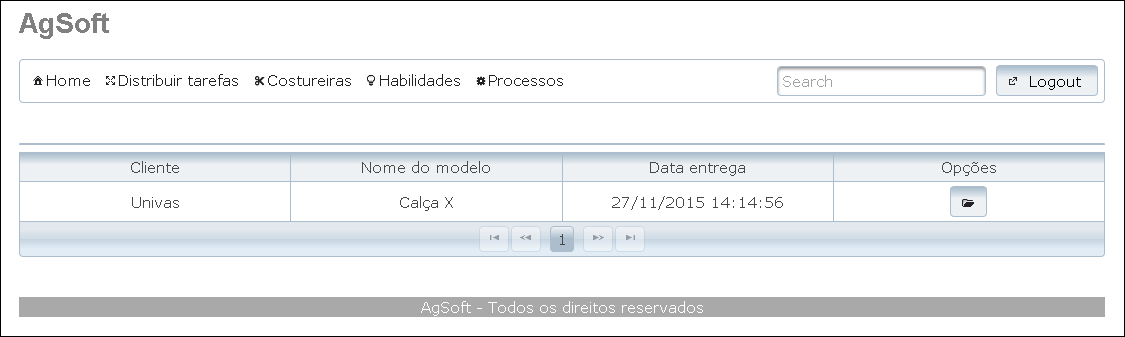
\includegraphics[scale=0.5]{./imagens/tela_distribuicao_processos.png}}
	\caption[Menu Distribuir tarefas]
	{Menu Distribuir tarefas
		\textbf{Fonte:} Desenvolvido pelos autores.}
	\label{fig:tela_dis_processos}
\end{figure}

\par Ao clicar no ícone "abrir", é aberta uma tela de distribuição para aquele processo, esta tela é responsável por captar alguns
dados importantes para a regra de negócio do algoritmo genético, além disto, é nela que as informações do melhor indivíduo (melhor
solução) são apresentadas.  Os dados informados através desta tela são o número total de peças que se deseja produzir, o número de 
peças que cada lote irá conter e a data de início da produção conforme mostra a Figura ~\ref{fig:tela_dis_open}.


\begin{figure}[h!]
	\centerline{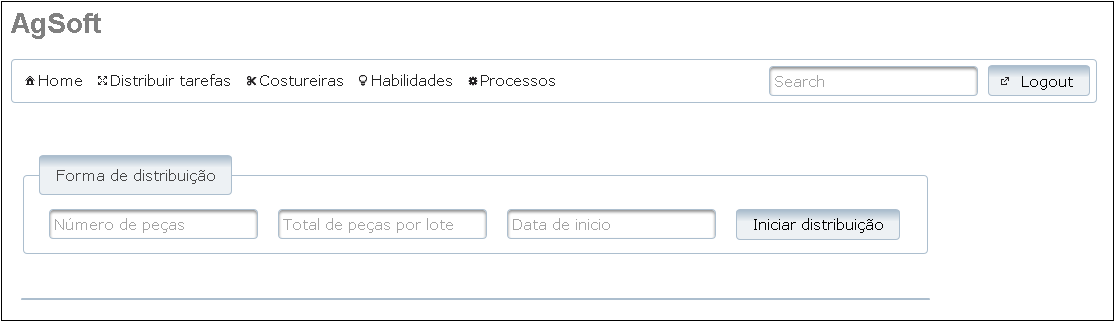
\includegraphics[scale=0.5]{./imagens/tela_distribuicao_open.png}}
	\caption[Tela de distribuição de tarefas]
	{Tela de distribuição de tarefas
		\textbf{Fonte:} Desenvolvido pelos autores.}
	\label{fig:tela_dis_open}
\end{figure}

\par Toda tela do criada com \texttt{JSF} é desenvolvida através de documentos \texttt{XHTML}, tais documentos possuem componentes para entrada e apresentação dos dados. Estes componentes podem ser tanto do \texttt{JSF} quanto do \textit{primefaces}, o Código ~\ref{list:metododoMutationOnChromossome} demonstra o documento \texttt{XHTML} da tela demonstrada acima.

\begin{lstlisting} [style=custom_Java,caption={[Método \texttt{doMutationOnChromossome()}]{Método \texttt{doMutationOnChromossome()}. \textbf{Fonte:} Elaborado pelos autores.}}, label=list:metododoMutationOnChromossome] 

<?xml version="1.0" encoding="UTF-8"?>
<ui:composition xmlns="http://www.w3.org/1999/xhtml"
xmlns:ui="http://java.sun.com/jsf/facelets"
xmlns:f="http://java.sun.com/jsf/core"
xmlns:h="http://java.sun.com/jsf/html"
xmlns:p="http://primefaces.org/ui">

<h:form id="formAbrirProcessoDis">
	<p:messages autoUpdate="true"></p:messages>
	
	<p:panelGrid columns="1">
	
		<div id="distribuicaoFields">
			<p:fieldset legend="Forma de distribuicao">
				<p:panelGrid columns="4">
					<p:inputText id="nPecas" required="true" 
					value="#{distribuicaoController.totalPecas}"
					requiredMessage="Por favor informe o total de pecas" 
					maxlength="19" placeholder="Numero de pecas" />
					
					<p:inputText id="totalPecaPorLote" required="true"
					value="#{distribuicaoController.totalPecasPorLote}"
					requiredMessage="Por favor informe o total 
						de pecas por lote"
						
					maxlength="19" placeholder="Total de pecas por lote"/>
					
					<p:calendar id="inicio" required="true"
								mask="true" effect="fold"
								value="#{distribuicaoController.dataInicio}"
								requiredMessage="Por favor informe uma data de inicio" 
								pattern="dd/MM/yyyy HH:mm:ss" 
									mindate="#{processosController.getCurrentDate()}"
					
								maxdate="#{distribuicaoController.getDataEntrega()}"
								placeholder="Data de inicio"/>
					
					<p:commandButton action="#{distribuicaoController.
						iniciarDistribuicao()}"
					
					value="Iniciar distribuicao" 
					update="formAbrirProcessoDis"
					ajax="true" onstart="PF('waitDialog').show();"
					onsuccess="PF('waitDialog').hide();"/>
				
				</p:panelGrid>
			</p:fieldset>
		</div>
	.
	.
	.

\end{lstlisting}

\par No \texttt{JSF}, toda página XHTML possui um controlador que consiste em uma classe Java, e para definir que tal 
classe é uma controladora de páginas, na sua declaração é definida a notação \texttt{@ManagedBean(name = "[nome da classe em minusculo]")}.
No caso da tela de distribuição, a classe controladora é denominada \texttt{DistribuiçãoController}, portanto possui a notação
\texttt{@ManagedBean(name = "[distribuiçãoController]")} em sua declaração. As páginas \texttt{XHTML} fazem então um \texttt{bind}, ou
seja, uma conexão com a classe controladora de forma que os dados do \texttt{XHTML} são disponibilizados em tal classe e vice-versa. 
No caso da página de distribuição, as \textit{tags} \texttt{<p:inputText} e \texttt{<p:calendar} são responsáveis pela entrada de 
informações, tais \textit{tags} possuem um atributo \texttt{value}, neste atributo é informado em qual classe controladora e em qual 
atributo desta os dados informados pelo usuário serão atribuídos, realizando assim o \textit{bind}, neste, caso os dados informados pelo 
usuário estarão respetivamente disponíveis nos atributos \texttt{totalPecas}, \texttt{totalPecasPorLote} e \texttt{dataInicio} da
classe \texttt{DistribuiçãoController}.

\par Após entrar com os dados necessários, o usuário deve clicar no botão Iniciar Distribuição, este botão é construído com a
\textit{TAG} \texttt{<p:commandButton} conforme mostra o Código acima. Esta \textit{TAG} possui o atributo \textit{action} que 
é responsável por chamar um método da classe controladora para executar uma determinada ação, neste caso, o método chamado é o 
\texttt{iniciarDistribuicao()} responsável por iniciar a distribuição das atividades chamando o gerenciador do algoritmo genético, 
conforme mostra o Código ~\ref{list:metodoiniciarDistribuicao}.

\begin{lstlisting} [style=custom_Java,caption={[Método \texttt{iniciarDistribuicao()}]{Método \texttt{iniciarDistribuicao()}. \textbf{Fonte:} Elaborado pelos autores.}}, label=list:metodoiniciarDistribuicao] 

public void iniciarDistribuicao(){
	int totalPecasInt = Integer.parseInt(totalPecas);
	int totalPecasPorLoteInt = Integer.parseInt(totalPecasPorLote);
	
	if(totalPecasInt == 0 || totalPecasPorLoteInt == 0){
		sendMessageToView(
			"Total de pecas ou total de pecas por lote e invalido!", 
				FacesMessage.SEVERITY_ERROR);
		return;
	}
	
	numeroDeLotes = totalPecasInt / totalPecasPorLoteInt;
	if((numeroDeLotes * totalPecasPorLoteInt) != totalPecasInt){
		sendMessageToView("Numero de lote nao exato: "+numeroDeLotes+" * "
			+ totalPecasPorLote+" = "+numeroDeLotes*totalPecasPorLoteInt, 
				FacesMessage.SEVERITY_ERROR);
		return;
	}
	
	if(idProcesso <= 0 || processo == null){
		sendMessageToView(
			"Processo invalido", FacesMessage.SEVERITY_ERROR);
		
		return;
	}
	
	prazEmSegundos = calcularPrazo();
	prazoAtendido = false;
	
	GeneticAlgorithmManagement gam = new GeneticAlgorithmManagement();
	melhorIndividuo = gam.iniciarDistribuicao(
		numeroDeLotes, prazEmSegundos, totalPecasPorLoteInt, idProcesso);
	
	//This is just to manage information messages in the view
	if(melhorIndividuo.getValue() <= prazEmSegundos.longValue()){
		prazoAtendido = true;
	}
	
	if(melhorIndividuo != null){
		rootFluxograma = construirArvore(melhorIndividuo.getNode(), null);
		allNodes = new ArrayList<Node>();
		rootTable  = 
			new DefaultTreeNode(
				new TabDetailBean("-", "-", "-","-","-","-","-"));
	
		construirTableDetail(melhorIndividuo);
		mostrarResult = true;
	}
}

\end{lstlisting}

\ Os dados que o algoritmo genético espera receber são número de lotes a serem distribuídos, o número de 
peças por lote e o prazo de entrega. Portanto uma das funções do método \texttt{iniciarDistribuicao()} é
calcular a quantidade de lotes a serem produzidos e o prazo de entrega das peças, além disto, o método 
realiza algumas validações, de forma a somente enviar informações consistentes para o algoritmo genético. 
O cálculo de número de lotes é realizado então dividindo o número de peças informado pelo usuário pelo 
número de peças por lote, o resultado é armazenado na variável \texttt{numeroDeLotes}.

\par Para calcular o prazo de entrega da produção é chamado o método \texttt{calcularPrazo()} demonstrado no 
Código ~\ref{metodoCalcularPrazo}.

\begin{lstlisting} [style=custom_Java,caption={[Método \texttt{calcularPrazo()}]{Método \texttt{calcularPrazo()}. \textbf{Fonte:} Elaborado pelos autores.}}, label=list:metodoCalcularPrazo] 

public BigDecimal calcularPrazo(){
	DateTime dataInical = new DateTime(dataInicio);
	DateTime dataFinal  = new DateTime(processo.getDataEntrega());
	return  new BigDecimal(Seconds.secondsBetween(dataInical, dataFinal).getSeconds());
}

\end{lstlisting}

\par É importante observar que o prazo é calculado em segundos, devido ao fato que o tempo de produção por peça e o tempo 
de transporte entre as costureiras são definidos em segundos. O método \texttt{calcularPrazo()} simplesmente retorna o tempo 
em segundos entre a data de início, informada pelo usuário e disponível no atributo \texttt{dataInicio} e o prazo de entrega, 
disponível no atributo \texttt{dataEntrega} do processo que foi informada no cadastro do mesmo. É importante ressaltar que
o objeto \texttt{processo} utilizado neste método foi criado no momento em que o usuário abriu o processo, neste caso, foi enviado
o \texttt{ID} do tal processo via \texttt{URL}e o controlador buscou, no banco, de dados as informações do mesmo através deste \texttt{ID}
criando assim tal objeto.

\par Após o calculo do número de lotes e do prazo, é instanciado um objeto da classe \texttt{GeneticAlgorithmManagement()}, conforme
explicado anteriormente, e então o método \texttt{iniciarDistribuicao()} é chamado. Tal método, conforme já visto nas seções anteriores
faz o gerenciamento da execução do algoritmo genético e retorna o melhor indivíduo encontrado, tal indivíduo é armazenado no 
atributo \texttt{melhorIndividuo} da classe \texttt{distribuiçãoController} e então os métodos \texttt{construirArvore()} e
\texttt{construirTableDetail()} são chamados para realizar a apresentação dos dados na tela após a distribuição, tais método
simplesmente pegam as atividades e suas respectivas costureiras juntamente com o número de lote que cada uma recebeu e 
apresenta ao usuário, além disto também é apresentado o tempo e o custo total, além de uma tabela de detalhes da distribuição.
A Figura ~\ref{fig:tela_dis_result} mostra a tela com o resultado da execução do algoritmo.

\newpage

\begin{figure}[h!]
	\centerline{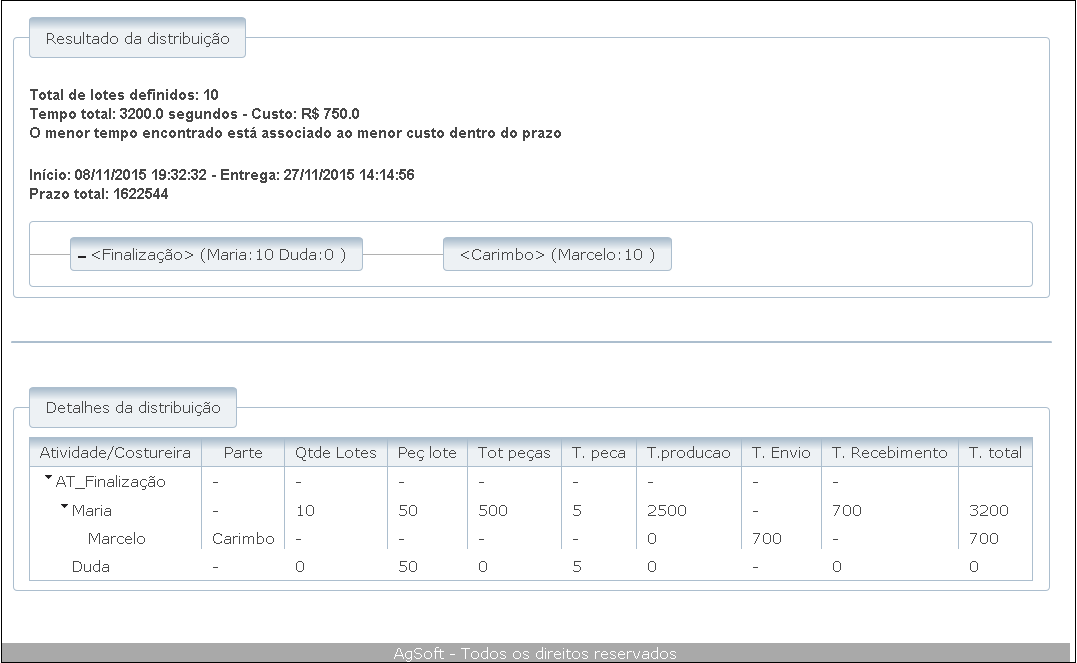
\includegraphics[scale=0.5]{./imagens/resultado_distribuicao.png}}
	\caption[Tela de resultado de distribuição de tarefas]
	{Tela de resultado de distribuição de tarefas
		\textbf{Fonte:} Desenvolvido pelos autores.}
	\label{fig:tela_dis_result}
\end{figure}

\par Os resultados serão vistos com mais detalhes nos casos de testes apresentados na discussão de resultados.

% \label{cap:quadroMetodologico}
% 
% \par Conteúdo do quadro metodológico. Perceba a forma que se coloca uma palavra entre aspas: o \LaTeX~oferece muita ``facilitade de formatação''.
% 
% Exemplo de código Java:
% 
% \begin{lstlisting} [style=custom_Java,caption={[Métodos da classe \texttt{FilmeBean}]{Métodos da classe \texttt{FilmeBean}. \textbf{Fonte:} Elaborado pelos autores.}}, label=fig:metodosclassebean] 	
% 	public FilmeBean(){  
%        //...
%    	}	
%    	
% 	public void saveMovie(){
% 		setListActorSelected();		
% 		if(this.movieDAO.saveMovieGraph(this.movieTo)){
% 			FacesContext.getCurrentInstance().addMessage(null, 
% 			   new FacesMessage("Filme cadastrado com sucesso!")); 
% 		}else{
% 			//...
% 		}		
% 		this.limpaCampos();
% 	}
% \end{lstlisting}
% 
% \par Agora será mostrado o exemplo do uso de fluxo de eventos apresentado no Quadro~\ref{quad:fluxo_evento_cadastro_filme}.
% 
% \begin{quadro}[h!]
%   \begin{fluxoDeEventos}
  \addTitle{Cadastrar filme}
  \addrow{Ator principal}{Administrador}
  %\addrow{Ator secundário}{Sistema de cartão}
  \addrow{Pré-requisitos}{Estar logado no sistema}

  \startBasicFlow{Ator} {Sistema}
  \addItemOne{Seleciona menu cadastro}
  \addItemOne{Clica na opção cadastrar filme}
  \addItemTwo{Abre interface de cadastro de filme}
  \addItemOne{Preenche formulário}
  \addItemOne{Clica no botão salvar}
  \addItemTwo{Salva e informa sucesso no cadastro}

  \startAlternativeFlow{Fluxo alternativo 1}
  \addItemOne{No item 5, formulário não preenchido}
  \addItemTwo{Exibe mensagem de necessidade de preenchimento de formulário}

  \startAlternativeFlow{Fluxo alternativo 2}
  \addItemOne{No item 6, inserido filme já cadastrado}
  \addItemTwo{Informa mensagem de filme já cadastrado}
\end{fluxoDeEventos}

%   \caption[Fluxo de eventos para cadastro de filme]
%            {Fluxo de eventos para cadastro de filme. \textbf{Fonte:} Elaborado pelos autores}
%   \label{quad:fluxo_evento_cadastro_filme}
% \end{quadro}
% 
% \par Outro exemplo é ilustrado na Figura~\ref{fig:bluesky}. Neste caso um código XML foi embutido dentro de um ambiente de figura, para que este código seja incluído no índice de figuras adequadamente.
%  
% \begin{figure}[ht!]
%   \begin{lstlisting} [style=custom_XML]
% 	...
% 	<context-param>
% 		<param-name>primefaces.THEME<\param-name>
% 		<param-value>bluesky<\param-value>
% 	<\context-param>
% 	...
%   \end{lstlisting}
%   \caption[Incluindo o tema \textit{BlueSky} ao contexto do projeto]
%           {Incluíndo o tema \textit{BlueSky} ao contexto do projeto. \textbf{Fonte:} Elaborado pelos autores.}
%   \label{fig:bluesky}
% \end{figure}
